%%%%%%%%%%%%%%%%%%%%%%%%%%%%%%%%%%%%%%%%%%%%%%%%%%%%%%%%%%%%%%%%%%%%%%%%%%%%%%%%%%%%%%%%%%%%%%%%%%%%%%%%%%%%%%%%%%%%%%%%%%%%%%%%%%%%%%%%%%%%%
\section{Introduction}\label{sec:ch6_intro}
%%%%%%%%%%%%%%%%%%%%%%%%%%%%%%%%%%%%%%%%%%%%%%%%%%%%%%%%%%%%%%%%%%%%%%%%%%%%%%%%%%%%%%%%%%%%%%%%%%%%%%%%%%%%%%%%%%%%%%%%%%%%%%%%%%%%%%%%%%%%%
In the previous section I have discussed the application of kicked optical potentials to vortex lattice-carrying Bose--Einstein condensates. The vortex lattice proved very resilient, with the perturbation not necessarily affecting the vortex positions, apart from some minor oscillations. The global structure of the lattice was preserved, and appeared well ordered. As the vortex lattice was largely unaffected by the optical lattice perturbation, it begs the question of how to create a disordered arrangement from this well ordered structure. Following from the similarity of vortex lattices to that of solid-state condensed matter materials, it is interesting to examine lattice ordering, and investigate behaviour of the vortices subjected to a defect or vacancy in the crystal structure. True crystalline solid-state materials have feature sizes on the order of {\AA}ngstroms, and can be difficult to observe experimentally, especially the appearance of lattice defects. Quantifying the disorder of vortex lattices has recently become an active topic of interest \cite{Vtx:Mithun_pra_2016,Rakonjac:16}. These topics are particularly useful as they can allow the study of quantum turbulence in highly controllable systems \cite{Vtx:Neely_prl_2013,Vtx:Kwon_pra_2014,Vtx:Groszek_pra_2016}.

Due to the topologically protected stability of the vortices, the vortex lattice itself is very robust to perturbations, as observed in the previous section. Unlike many solid-state materials, the vortex lattice can be directly manipulated, allowing for an investigation into order-disorder effects.  An interesting question to ask, builidng upon these works, is if the lattice were to lose a vortex at a specified location, how would the overall system respond? While this method is mostly inaccessible in solid-state systems, I propose here using the phase imprinting technique to investigate this type of behaviour in a vortex lattice carrying condensate.

In Section~\ref{sec:phase} I discussed the use of phase imprinting techniques to modify the condensate phase to a deserved form. While it was discussed that a vortex can be created with the required $\pm 2\pi$ phase winding, it can also be used to annihilate a vortex of pre-existing winding. Assuming a vortex with clockwise phase winding, the direct application of an antivortex with counter-clockwise winding can remove this topological charge of the vortex and annihilate it. In this chapter I will examine the use of this technique, and investigate the resulting effect on the vortex lattice order.



This work is submitted for publication to PRA, with content referenced therefrom.


%%%%%%%%%%%%%%%%%%%%%%%%%%%%%%%%%%%%%%%%%%%%%%%%%%%%%%%%%%%%%%%%%%%%%%%%%%%%%%%%%%%%%%%%%%%%%%%%%%%%%%%%%%%%%%%%%%%%%%%%%%%%%%%%%%%%%%%%%%%%%
\section{Model}\label{sec:model}
%%%%%%%%%%%%%%%%%%%%%%%%%%%%%%%%%%%%%%%%%%%%%%%%%%%%%%%%%%%%%%%%%%%%%%%%%%%%%%%%%%%%%%%%%%%%%%%%%%%%%%%%%%%%%%%%%%%%%%%%%%%%%%%%%%%%%%%%%%%%%

To investigate the evolution of the vortex lattice subjected to the phase imprinting technique I once again numerically solve the Gross--Pitaevskii equation in two dimensions, assuming a strong confinement along the third axis, following the model given in Sec.~\ref{sec:modelsystem}. This allows me to restrict the dynamics to the $x$--$y$ plane and focus fully on the Abrikosov lattice geometry. Experimentally, this corresponds to a system with a very strong confinement in one direction only \cite{BEC:Stock_lpl_2004,BEC:Seo_jkps_2014,BEC:Chomaz_natcom_2015} and in the frame co-rotating with the condensate, the non-linear mean field equation governing the BEC wave-function is once again given by
\begin{align}
	i\hbar\partial_t \Psi(\mathbf{r},t) = \Big[&-\frac{\hbar^2}{2m}\nabla^2 + V\left(\mathbf{r}\right) \nonumber\\
	&+ g\vert \Psi(\mathbf{r},t) \vert^2- \Omega L_z \Big]\Psi(\mathbf{r},t).
\end{align}
%Here $V\left(\mathbf{r}\right)$ is the harmonic trapping potential with a frequency $\omega_\perp=2\pi\times1$ Hz. The trap rotation frequency is given by $\Omega$ and $L_z$ is the angular momentum operator along the $z$-direction. The effective interaction strength in 2D is characterized by $g$ and we assume to have $N=9.8\times 10^5$ atoms of $^{87}$Rb, with a singlet state \textit{s}-wave scattering length of $a_s = 90r_b \approx 4.76\times 10^{-9}$ m, where $r_B$ is the Bohr radius. For the rapidly rotating case, $\Omega=0.995\omega_\perp$, the vortices form an ordered triangular lattice with spacing $a_0 \approx 2.1\times 10^{-5}$ m, that rotates similarly to a solid-body in the large number limit \cite{BEC:Fetter_rmp_2009}.

To quantify the order of the vortex lattice the position of each vortex was found by summing the wavefunction phase over adjacent grid sites, and looking for a $2\pi$ winding. This gave a vortex position estimated to the numerical grid. A least-squares fit was then performed to more accurately determine the vortex core to sub-grid resolution. As tracking many-body dynamics is a complex problem, I make use of the Delaunay triangulation technique from computational geometry to examine the ordering of the the vortex lattice, as discussed in Sec.~\ref{sec:delaunay}. In the ideal triangular Abrikosov lattice, every vortex has 6 nearest neighbors, $l=\{0,\ldots,5\}$, located at $\theta_l=l\pi/3$ around the polar angle and any perturbation related to a defect changes these locations. Delaunay triangulation generates a mesh from the vortex positions, which makes it easy to check for the presence of non 6-fold connected vortices. These vortices are termed as $n$-fold topological lattice defects, where $n$ is the number of connected edges, and dislocation defects can form when, for example, a 5-fold and a 7-fold defects pair. Since all these structures are easily countable, this method allows us to characterize the effect a well-defined perturbation has on the lattice.

As unperturbed Abrikosov lattices in BECs are well ordered everywhere in the bulk region \cite{Vtx:Anglin_arxiv_2002} we define a radial boundary at approximately $2/3$ of the maximum density, which corresponds to $r_v=2\times 10^{-4}$ m from the center and restrict our analysis to vortices inside it. This leaves an edge boundary of approximately $4a_0$ wide where vortices are not counted. For the coordinate locations of each vortex within the boundary, it is possible to calculate statistical quantities of the resulting lattice quality. As our system is of finite size, the usually used translational correlations have only limited value and we will focus in the following on orientational correlations, which quantify how the lattice aligns along a particular angle. The orientational correlation function is defined as
\begin{align}
	g_6(r) = \frac{1}{N(r)}\displaystyle\sum\limits_{j,k}^{N(r)}\zeta_6(\mathbf{r}_j)\zeta_6^{*}(\mathbf{r}_k),
\end{align}
with
\begin{align}
	\zeta_6(\mathbf{r}_{j}) =  \frac{1}{n_j}\displaystyle\sum\limits_{l}^{n_j}\exp(\mathrm{i}6\theta_{jl}),
\end{align}
where $N(r)$ is the number of paired vortices separated by $r=|\mathbf{r}_j - \mathbf{r}_k|$, $\zeta_6$ is the orientational order parameter, $l$ runs over the nearest neighboring vortices, and $\theta_{jl}$ is the angle a paired vortex and nearest neighbor makes relative to a reference axis \cite{Guillamon_nat_2014}. We examine the orientational correlation function as a measure of the order of a ``vortex unit cell'', defined by the angle made by nearest neighbors to an individual vortex. For a perfectly ordered triangular lattice this value will tend to 1 at crystal structure spacings, and 0 elsewhere.

%%%%%%%%%%%%%%%%%%%%%%%%%%%%%%%%%%%%%%%%%%%%%%%%%%%%%%%%%%%%%%%%%%%%%%%%%%%%%%%%%%%%%%%%%%%%%%%%%%%%%%%%%%%%%%%%%%%%%%%%%%%%%%%%%%%%%%%%%%%%%
\section{Phase imprinting defects}\label{sec:phase}
%%%%%%%%%%%%%%%%%%%%%%%%%%%%%%%%%%%%%%%%%%%%%%%%%%%%%%%%%%%%%%%%%%%%%%%%%%%%%%%%%%%%%%%%%%%%%%%%%%%%%%%%%%%%%%%%%%%%%%%%%%%%%%%%%%%%%%%%%%%%%

[discussed earlier - pull more from paper]

\subsection{Single vortex dynamics}

To fully understand the effects of removing a vortex from the lattice system, I will first investigate the situation where the vorticity from a condensate carrying only a single vortex is removed. For this I apply a phase pattern that exactly cancels the $2\pi$ phase winding and simulate the resulting dynamics. The results of such a process can be seen in Fig.~\ref{fig:annihilation_1vtx}, and, as expected, the depletion in the condensate density fills in after the vortex phase is removed and the breathing mode is excited. Since the system is rotationally symmetric, we also plot the expectation value of the squared radius, $\langle r^2 \rangle$, where $r^2 = x^2 + y^2$, which clearly shows that the annihilation process excites the breathing mode at the expected frequency of $2\omega_\perp$ for a two-dimensional system \cite{BEC:Pitaevskii_pra_1997}. The change in energy due to the phase removal can be meaningfully characterised via the ratio of compressible (phonon) and incompressible (vortex) kinetic energy as given by Sec.~\ref{sec:kinspec}, with the spectra shown in Fig.~\ref{fig:kinspec}. As a reminder for the reader the kinetic energies are determined from the density weighted velocity field, $\mathbf{u} = |\Psi|\frac{\hbar}{m}\nabla \theta$, where $\theta$ is the phase of the condensate. The contribution from the compressible and incompressible energies can be taken as $\mathbf{u} = \mathbf{u}^{c} + \mathbf{u}^{i}$, and are determined by solving
\begin{subequations}
    \begin{align}
        \nabla \times \mathbf{u}^{c} = 0 \\
        \nabla \cdot \mathbf{u}^{i} = 0.
    \end{align}
\end{subequations}
The resulting spectra, $E^{i,c}$, are then calculated as an angle average over binned magnitudes in reciprocal space \cite{CT:Bradley_prx_2012}
\begin{equation}
    E^{i,c}(k) = \frac{mk}{2}\displaystyle\sum_{j\in r}\int\limits_{0}^{2\pi} d\phi_k \frac{\mathcal{U}^{i,c}_j(\mathbf{k},t)}{s_k},
\end{equation}
where
\begin{equation}
    \mathcal{U}^{i,c}_{j}(\mathbf{k},t) = \int d^2\mathbf{r}e^{-\text{i}(\mathbf{k}\cdot \mathbf{r})}u_j^{i,c}(\mathbf{r},t).
\end{equation}
As one can see from Fig.~\ref{fig:kinspec} after the vortex is annihilated and sounds wave are created, the energy ratio drops and lower incompressible-to-compressible values appear, in particular for higher wavenumbers. The latter is due to the removal of large kinetic energies from the atoms close to the vortex core.

\begin{figure}[h!]\centering
    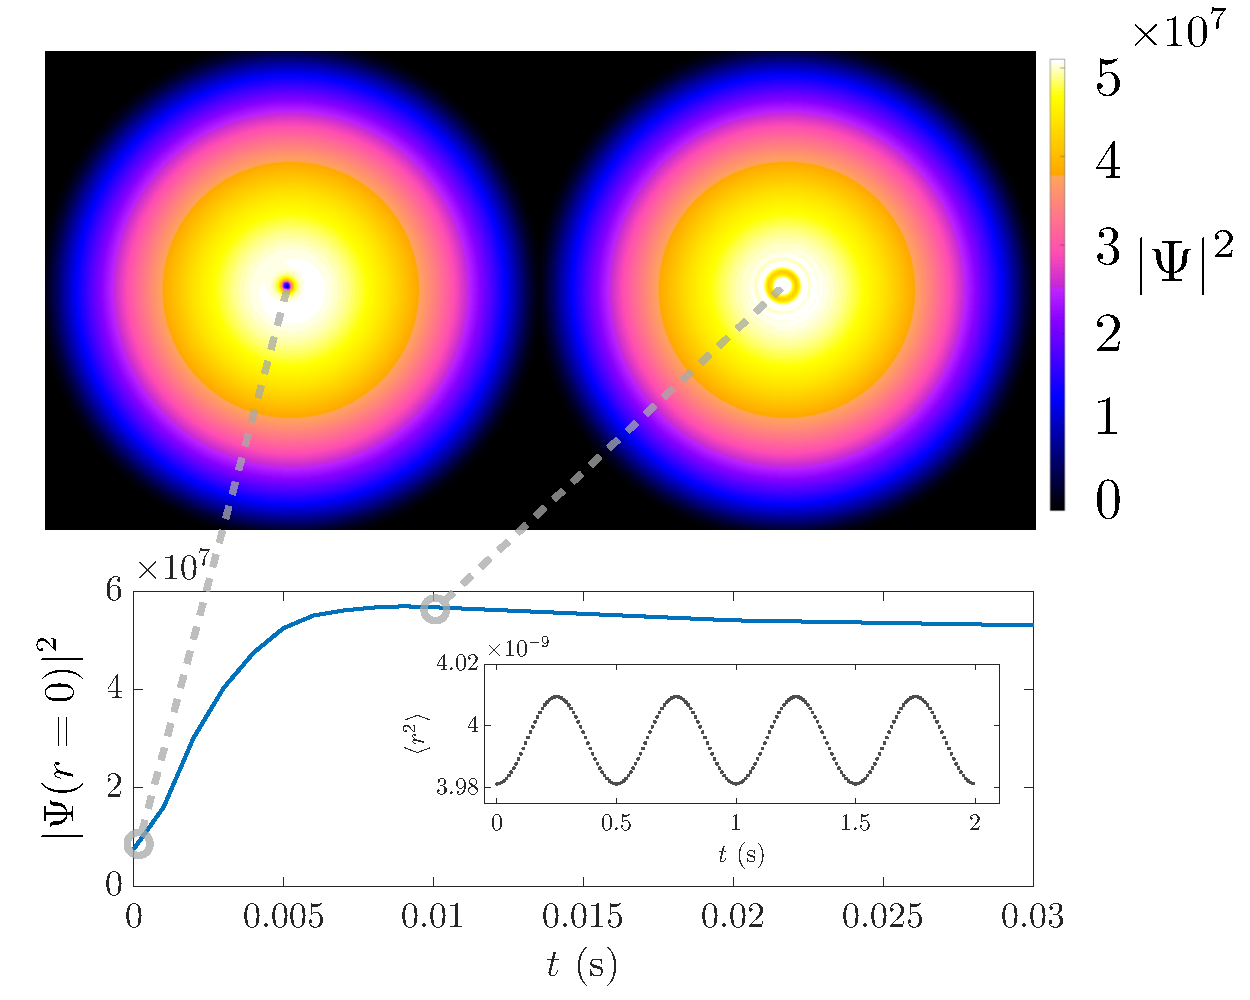
\includegraphics[width=0.7\textwidth]{ch6_phasegineer/arxiv/fig1.pdf}
    \caption{The evolution of the condensate density is shown for the initial state, and after 10 ms of evolution. The removal of the phase singularity at $r=0$ leads to a filling in of the density dip, which can also be seen from the line-plot. The process excites the monopole mode at frequency $2\omega_\perp$ (see inset).}\label{fig:annihilation_1vtx}
\end{figure}
\begin{figure}[h!]\centering
    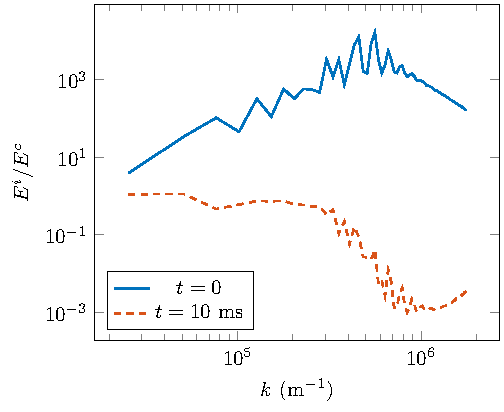
\includegraphics[width=0.7\textwidth]{ch6_phasegineer/arxiv/fig2.pdf}
    \caption{Ratio of incompressible to compressible energy at  $t=0$ (solid) and $t=10$ ms (dashed). Initially the incompressible energy is greater than the compressible due to the presence of the vortex, giving values greater than unity for all $k$. After application of the phase profile, the vortex is annihilated, with the energy released as phonons, indicated by a decrease in incompressible energy for all $k$ values.}\label{fig:kinspec}
\end{figure}

While the above example suggests that erasing vortices is a straightforward and controllable process, this assumption needs to be checked for the situation where the imprinted phase and the existing phase are not perfectly centered on each other. This situation is shown in Fig.~\ref{fig:annihilation_1vtx_uncentred}, and one finds that cases where the imprinted profile is sufficiently close to the core (i.e. within a healing length) the existing vortex gets erased as before. However, beyond this distance a separate antivortex gets created and the vortex-antivortex pair travels to the edge of the condensate system and begins to circulate around \cite{VTX:Martikainen_pra_2001}. For a densely packed lattice of vortices, however, this is not a problem since the typical distance between vortices is of the same order of magnitude as the healing length.

\begin{figure}[h!]\centering
    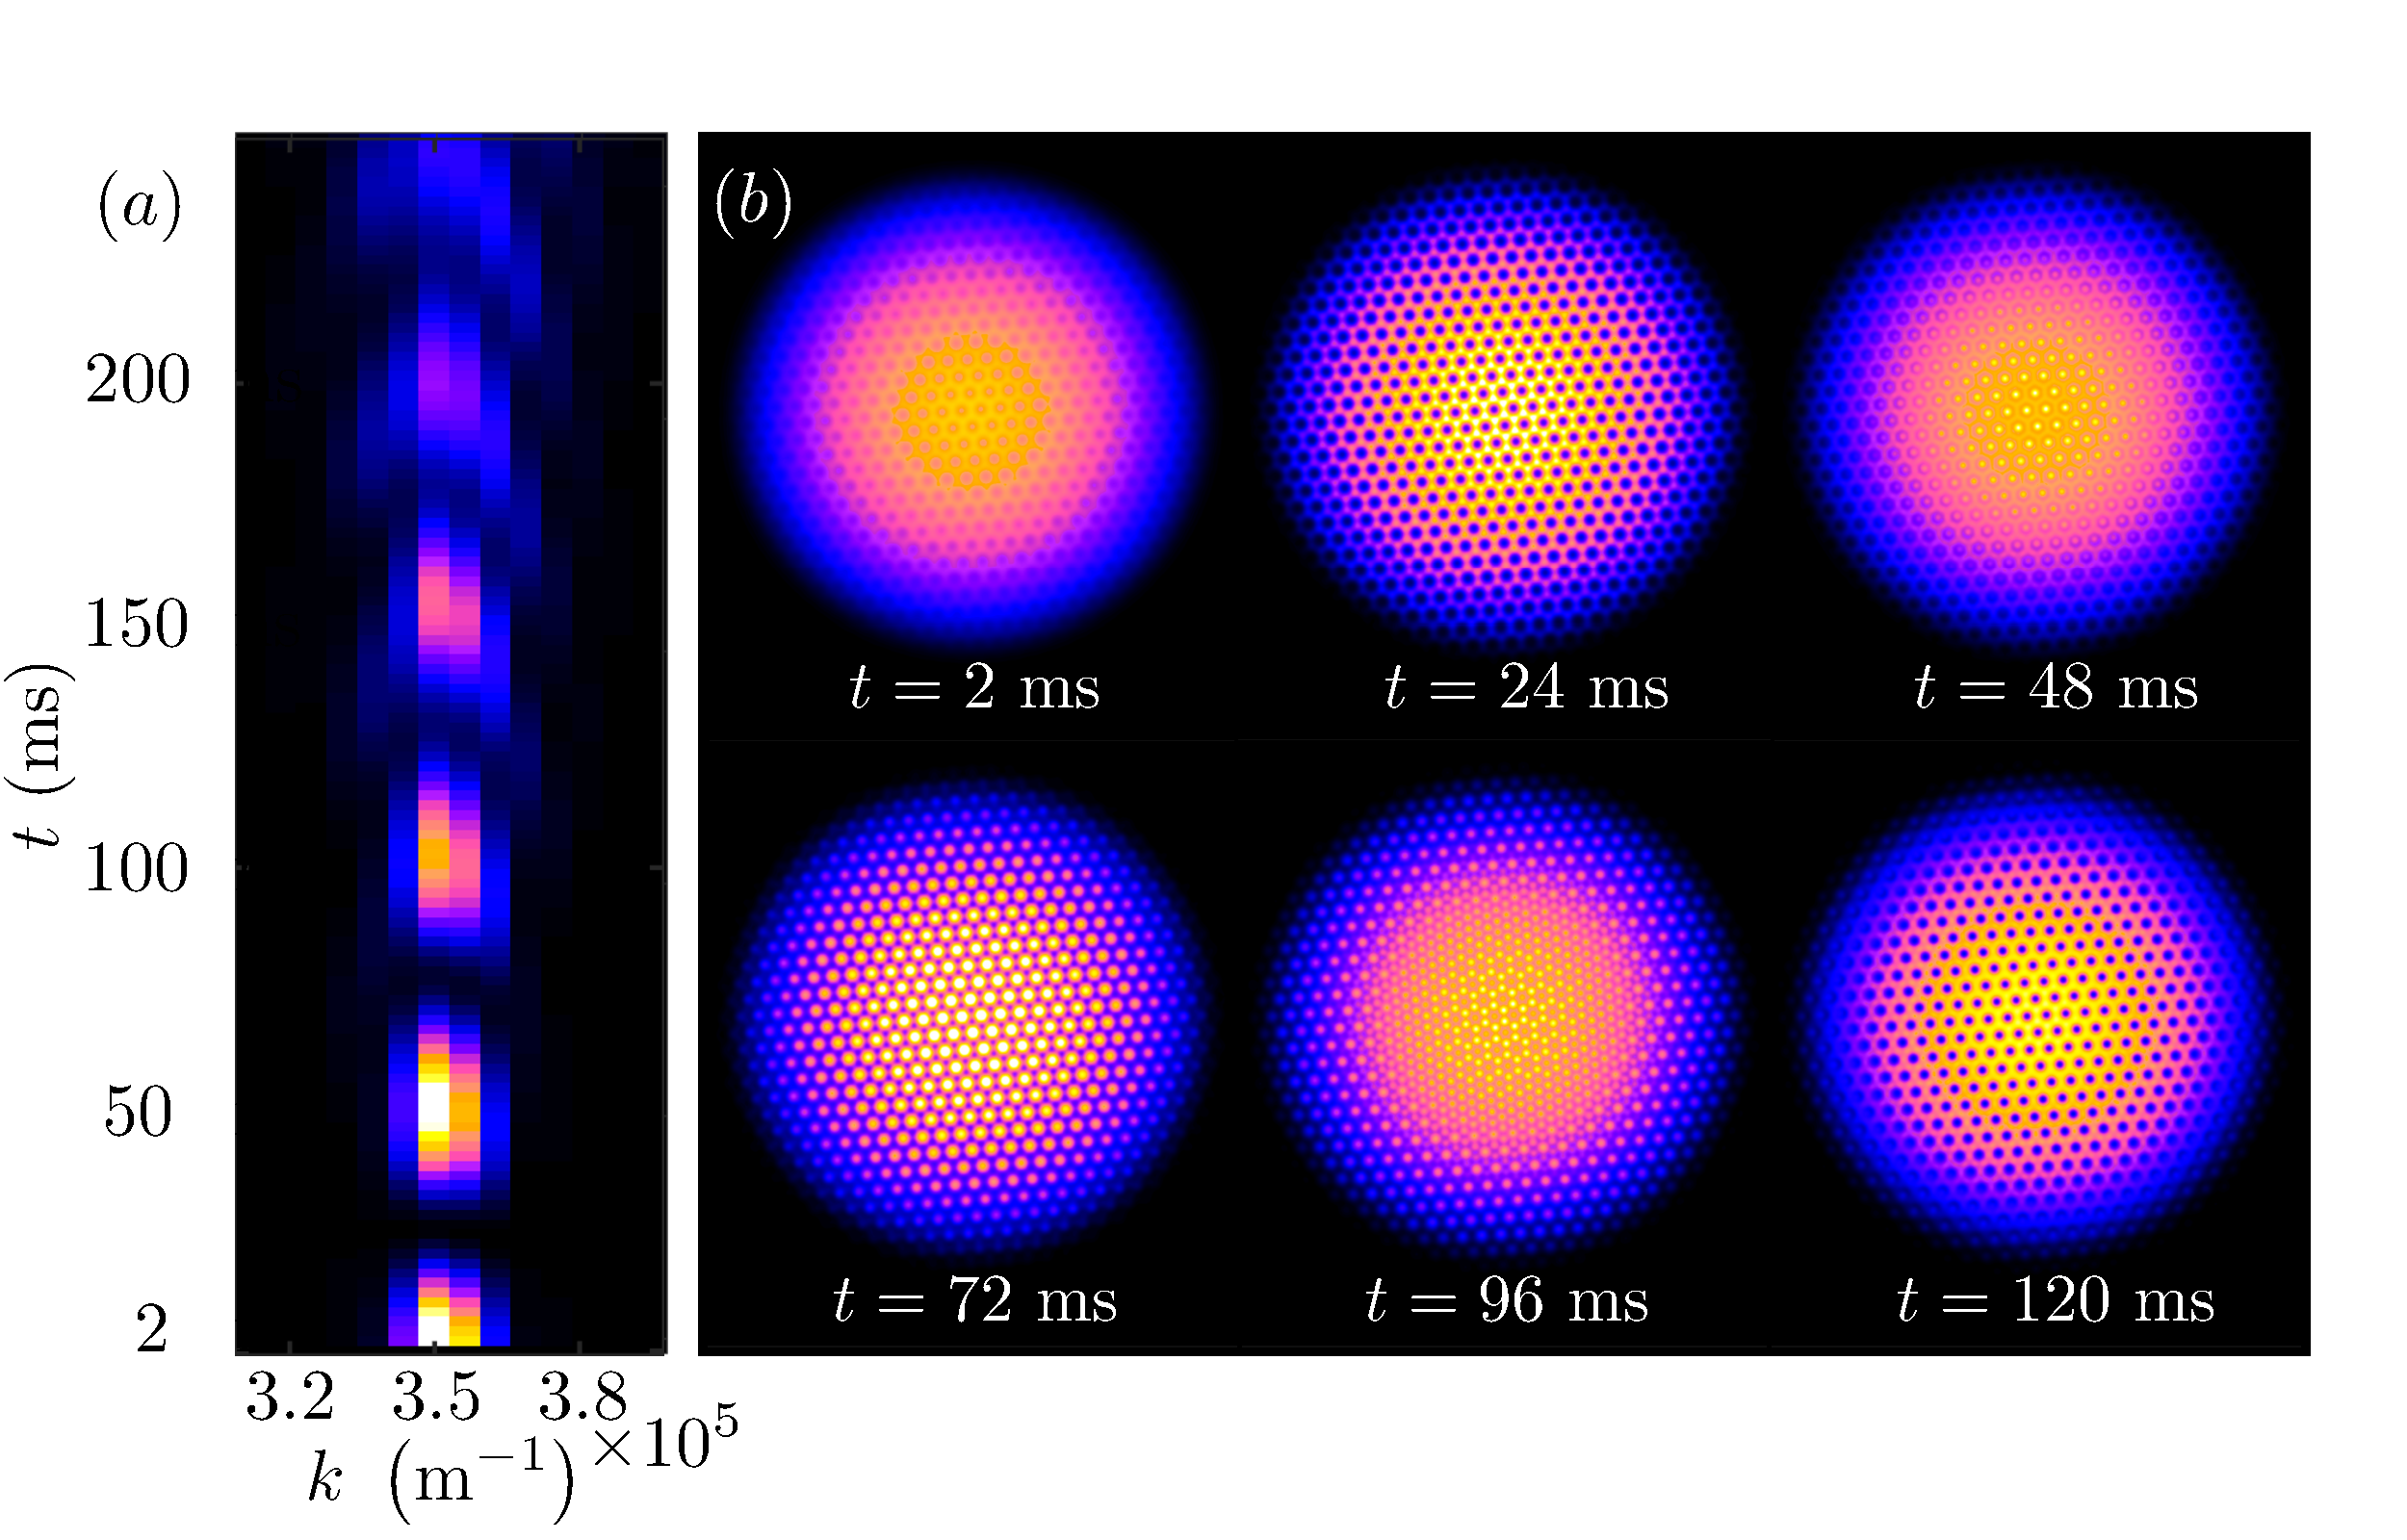
\includegraphics[width=0.7\textwidth]{ch6_phasegineer/arxiv/fig3.pdf}
    \caption{The condensate evolution following an uncentered phase imprint. For an imprint where the singularities of the vortex and the imprinted phase are less than a healing length away from each other, the existing vortex is annihilated and phonon modes are excited (a,b). However, beyond this distance an antivortex is created, which travels with the pre-existing vortex and circulates the condensate (c,d,e).}\label{fig:annihilation_1vtx_uncentred}
\end{figure}


\subsection{Lattice dynamics}

%%%%%%%%%%%%%%%%%%%%%%%%%%%%%%%%%%%%%%%%%%%%%%%%%%%%%%%%%%%%%%%%%%%%%%%%%%%%%%%%%%%%%%%%%%%%%%%%%%%%%%%%%%%%%%%%%%%%%%%%%%%%%%%%%%%%%%%%%%%%%

The removal of a single vortex from the vortex lattice by phase erasing initially affects only the nearest neighbors, as the phase gradient is only significant over the length scale of a healing length close to the erased singularity. The altered velocity profile will lead to the remaining vortices leaving their position in the Abrikosov lattice and the excitation of phonon modes. However in the lattice areas away from the impurity, these phonon modes have only minimal impact on the geometry \cite{VTX:oriordan_pra_2016}. To characterize the vortex dynamics following the application of the phase profile, we will in the following track each individual vortex throughout the full time-evolution and use the resulting trajectories and Delaunay triangulation for analysis.

\begin{figure}[h!]\centering
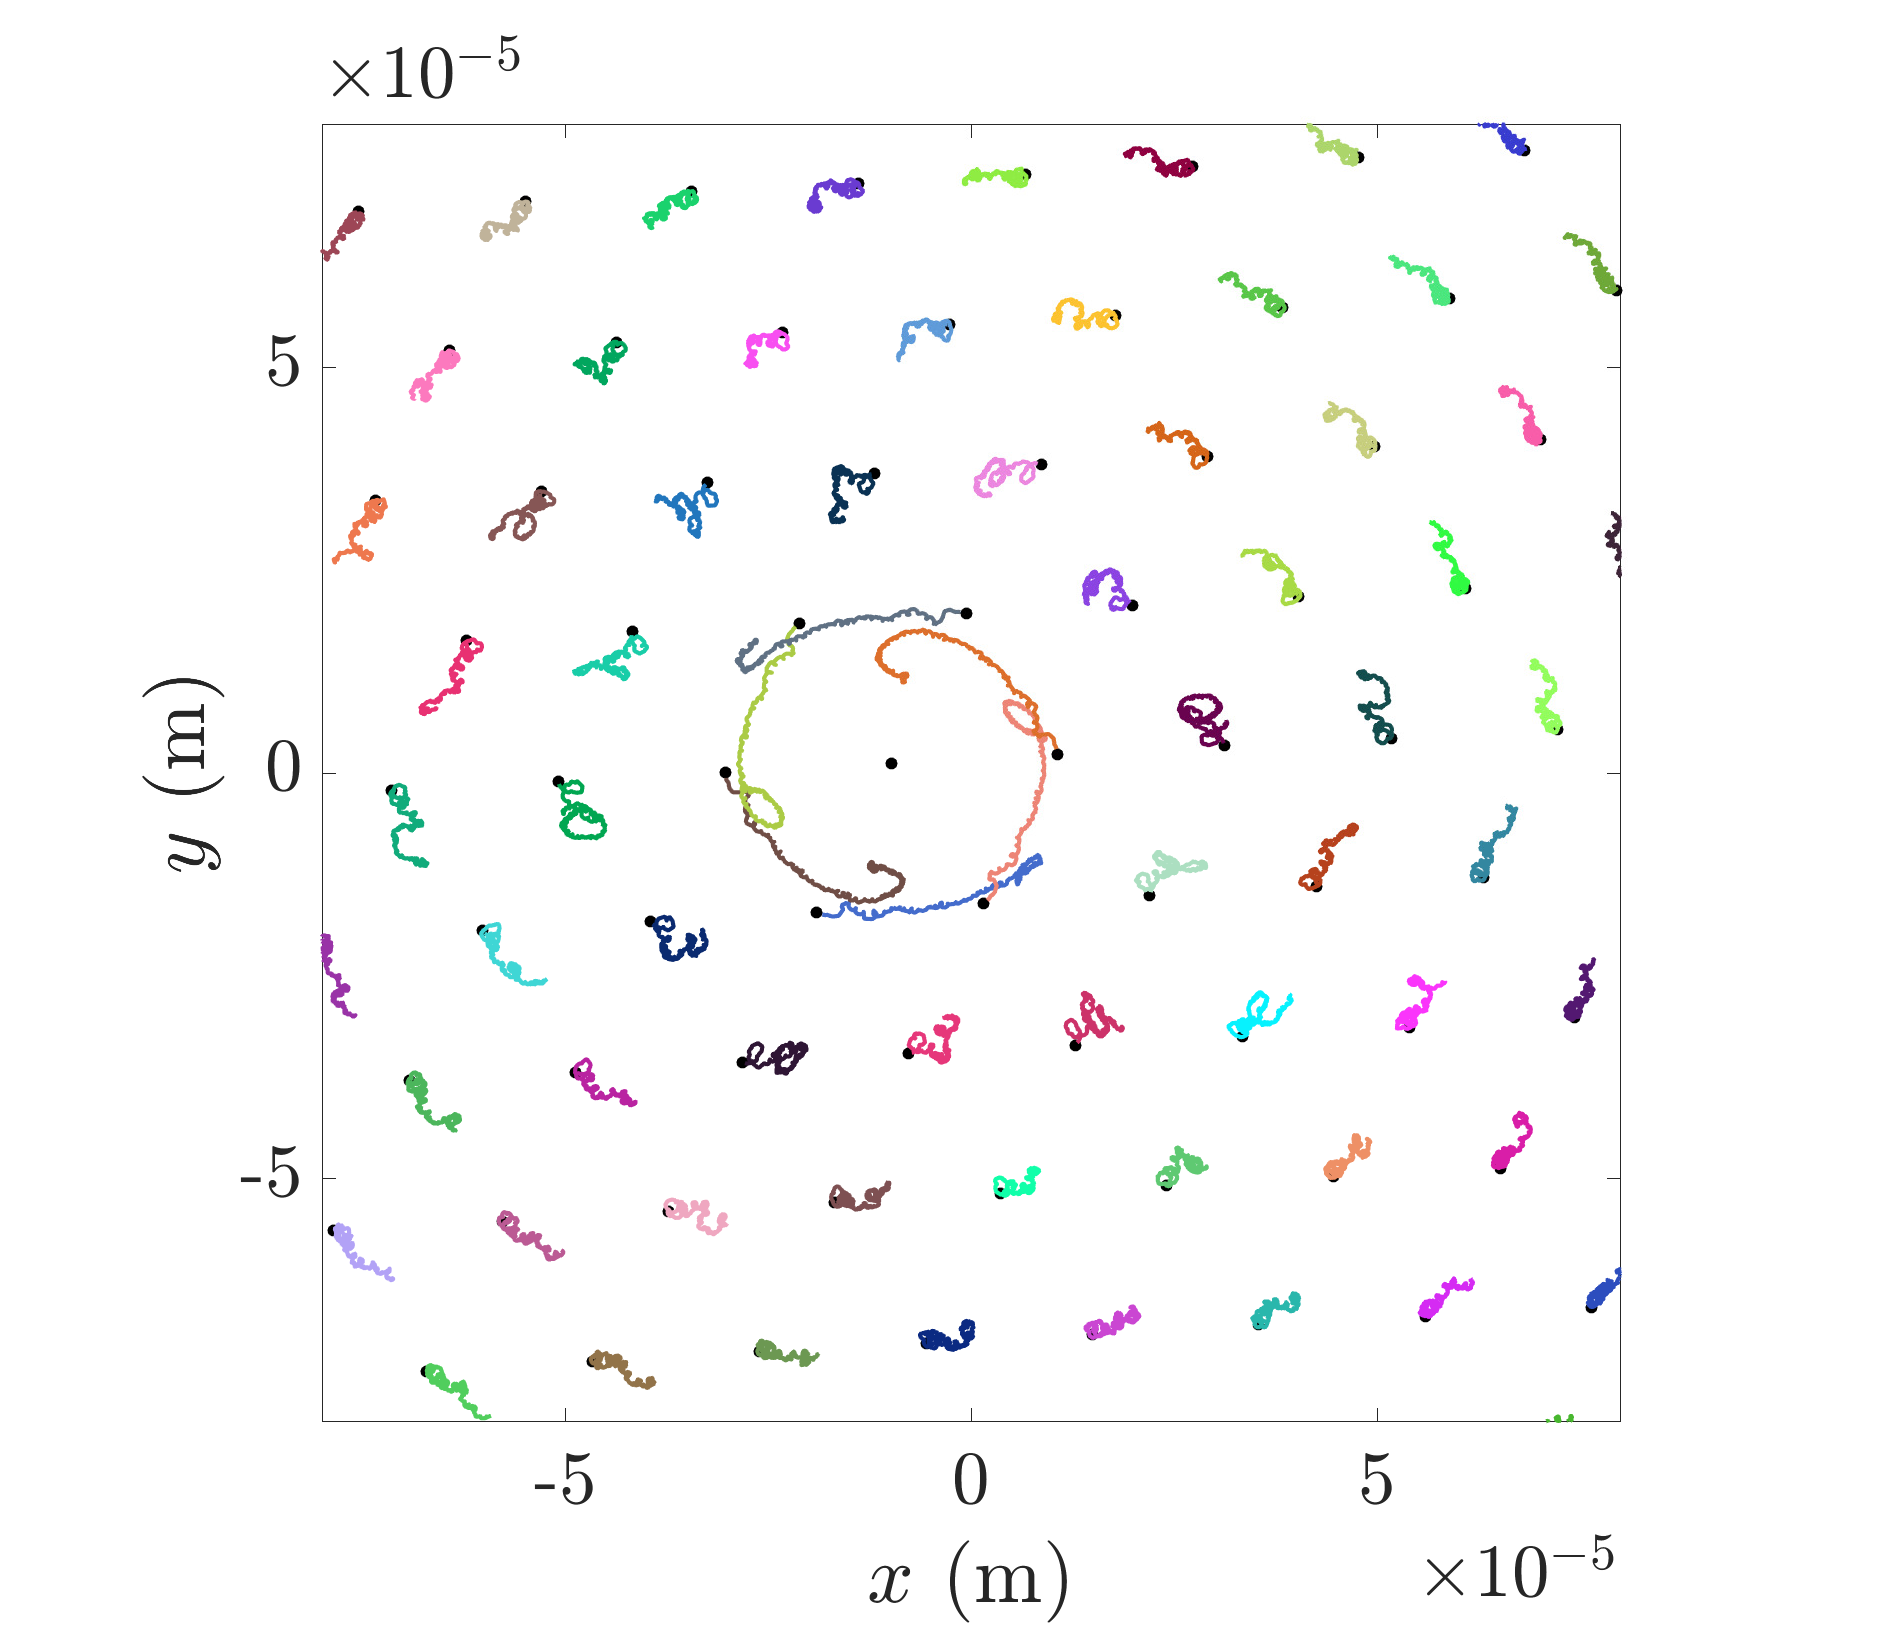
\includegraphics[width=0.7\textwidth]{ch6_phasegineer/arxiv/fig4.pdf}
    \caption{The trajectories of the vortices over 4 seconds following the removal of the vortex closest to the center, where each color represents a unique trajectory path. The vortices can be seen to move counter-clockwise in the co-rotating frame due to the loss of the local velocity field. However, the effect of the removal decreases quickly with increased radial distance. }
    \label{fig:trajplot}
\end{figure}

Let us first consider the situation where a single vortex is erased within the central area of the vortex lattice. In Fig.~\ref{fig:trajplot} we show the trajectories of the remaining vortices over a time-scale of 4 seconds. One can see that a long-lived vacancy is maintained close to the centre with the adjacent vortices rotating faster than the lattice due to the loss of the local velocity field, as is shown by Fig.~\ref{fig:velocityfield_ch6}. The honeycomb-like vacancy region eventually decays and the system settles into a new local geometry. Very similar behavior can be observed if the erased vortex is not one of the central ones, as long as it is within a region of constant areal vortex density. However, being closer to the edge of the lattice reduces the stability of the perturbed region. The overall lattice remains well structured after a vortex removal, as can be seen from the orientational correlation function shown in Fig.~\ref{fig:g6} for different times. Although the gaps between the peaks that exist at $t=0$ disappear during the evolution due to the presence of the phonon excitation, the overall correlations remain high for long times and constant across all length scales. The slight peak softening arises from the vortices no longer being aligned to a perfect triangular lattice position, which is indicative of a weak disordering or distortion of the lattice structure.

\begin{figure}[h!]\centering
    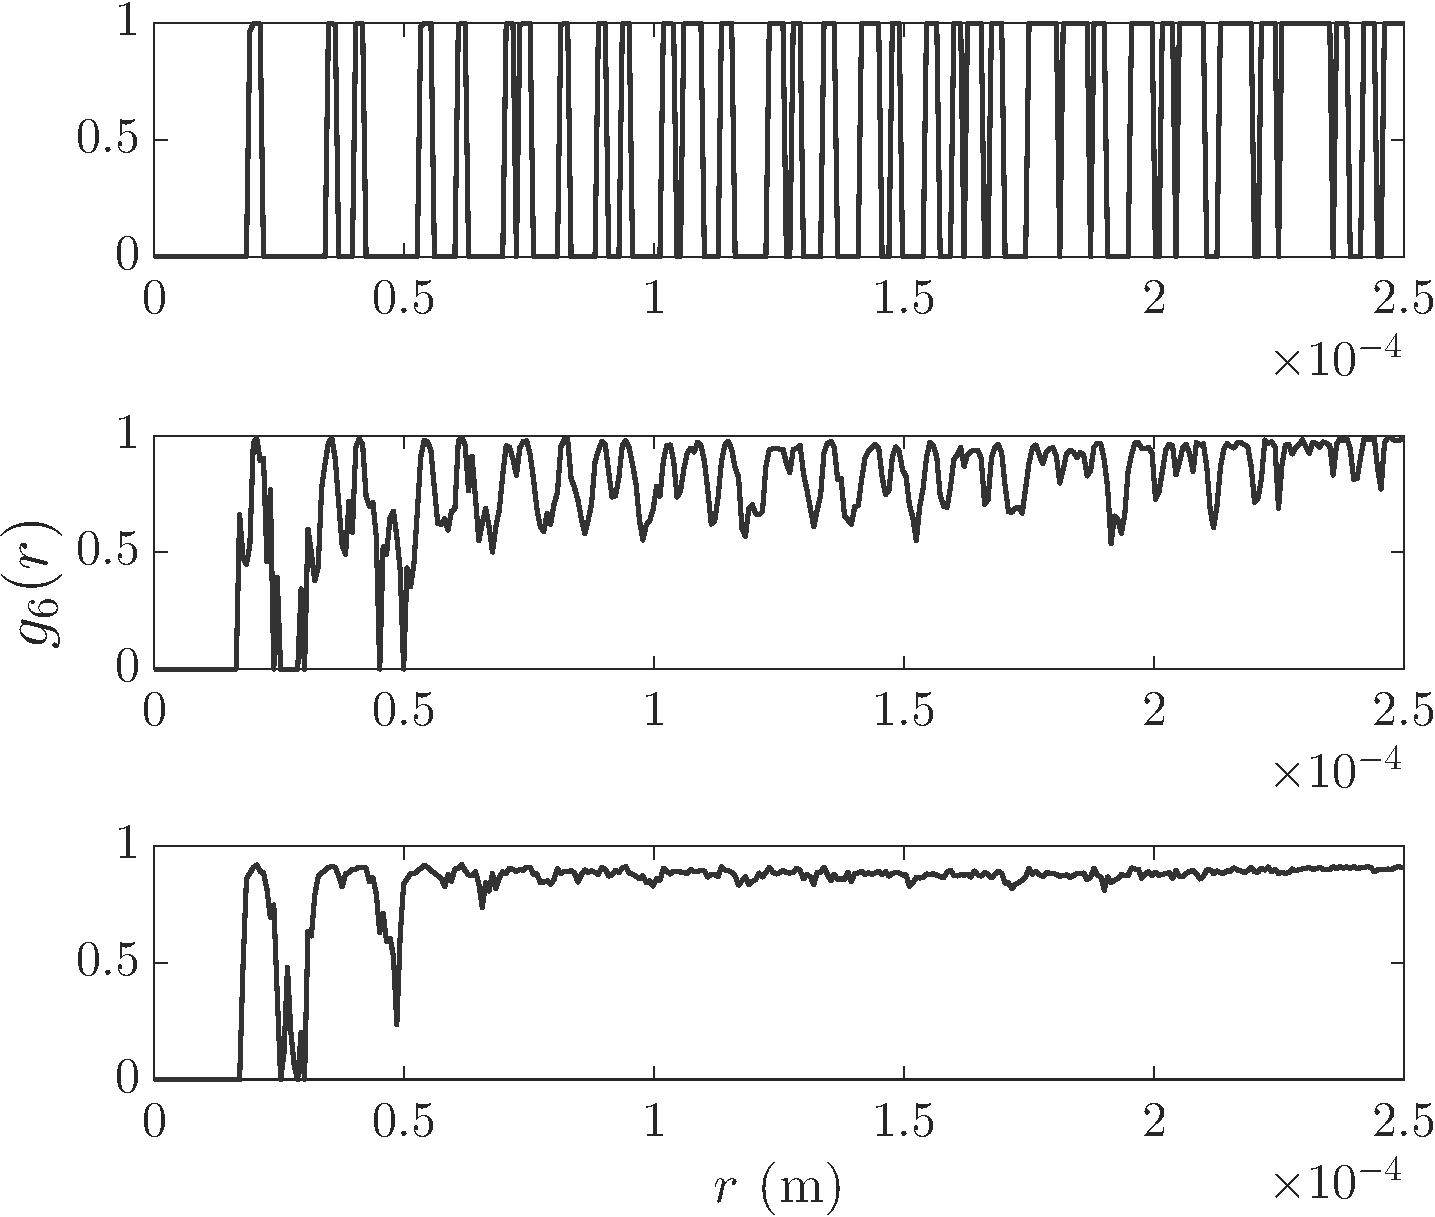
\includegraphics[width=0.7\textwidth]{ch6_phasegineer/arxiv/fig5.pdf}
    \caption{The orientational correlation function for the vortex lattice after removing the central vortex is given for $t=\{0,1,6\}$ seconds (top to bottom). The peaks at $t=0$ appear at nearest neighbor, next nearest, and higher order distances. Due to finite binning of the lengths, the peaks become grouped to 1 at higher length scales. For times greater than $t=0$, the peak correlations drop, however, the large value at long times indicates a well ordered lattice as high correlations are observed across all length scales.}\label{fig:g6}
\end{figure}

As described above, the Delaunay triangulation of the lattice can give a graphical overview of how connected the different vortices are, and therefore what changes to the lattice structure have occurred \cite{Guillamon_nat_2014}. We show the resulting graph for the case where a single vortex was removed from the center of the lattice in Fig.~\ref{fig:deltri_1vtx}. One can see that a pair of (5,7)-fold connected lattice defects form after the removal (at 10 ms), which slightly adjusts and becomes stable for long times. Removing vortices at different positions in the lattice shows similar behavior, with a localization of the disordered region not far from the site of vortex removal.

\begin{figure}[h!]\centering
    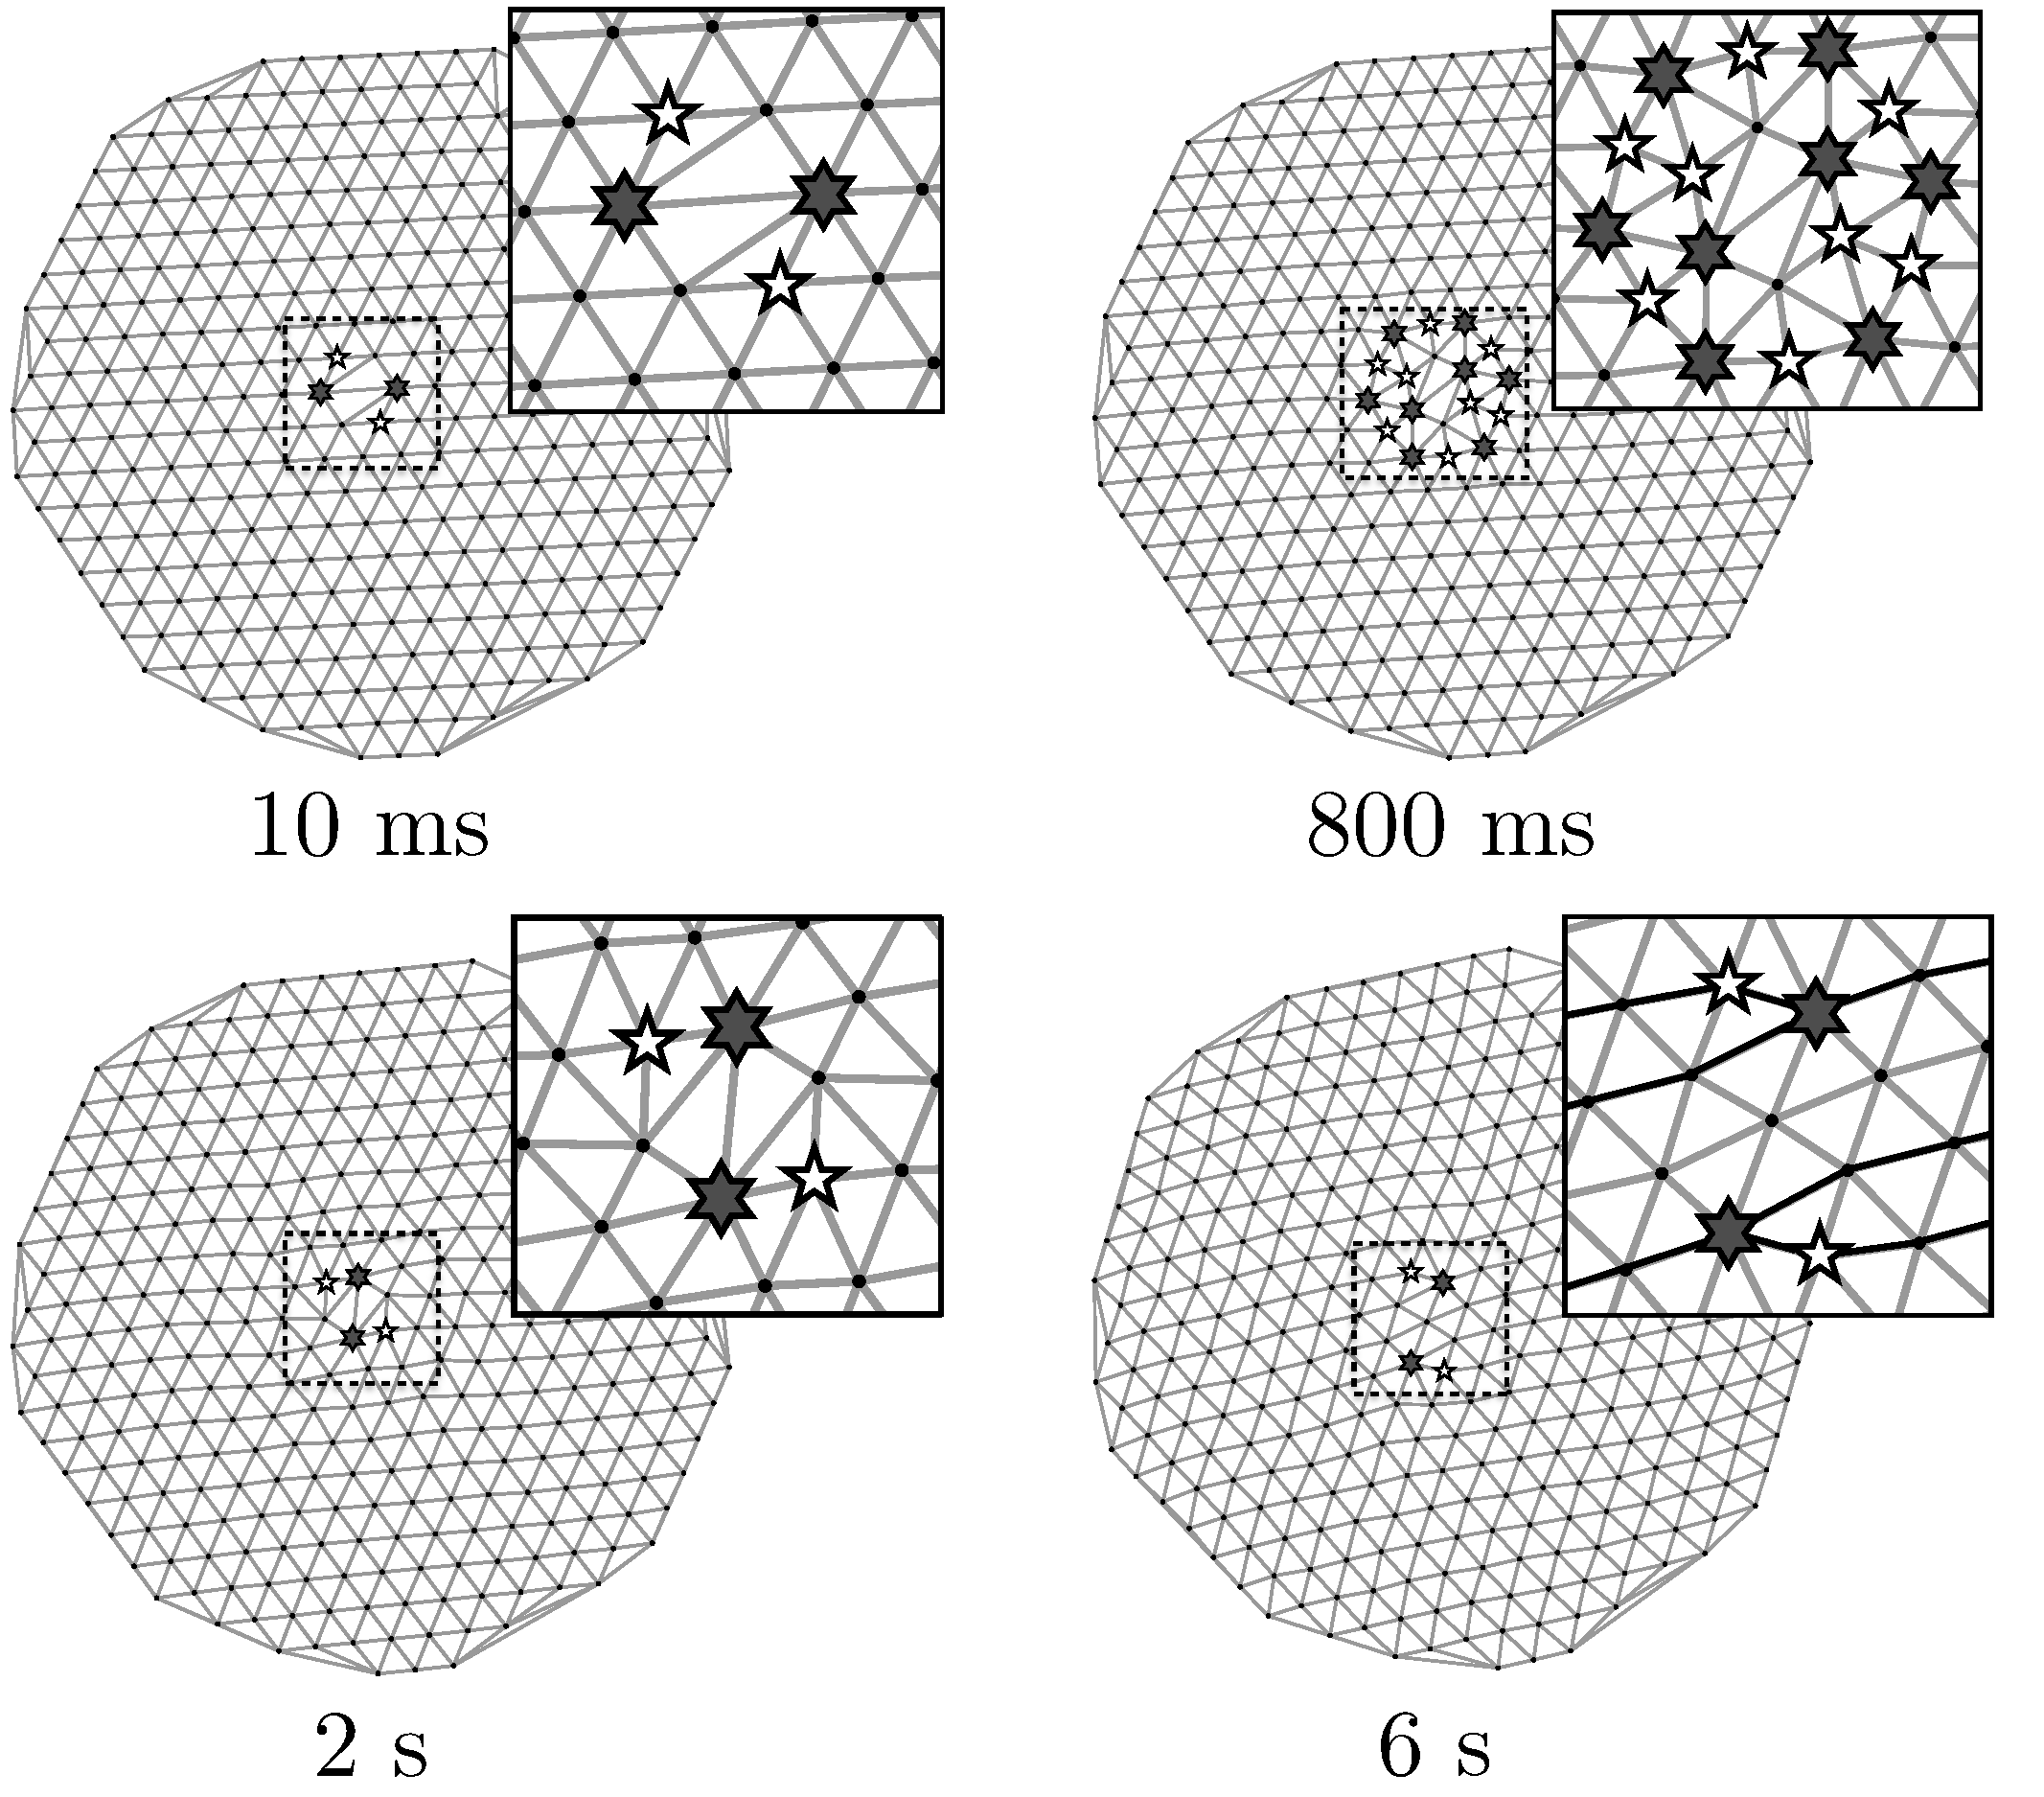
\includegraphics[width=0.7\textwidth]{ch6_phasegineer/arxiv/fig6.pdf}
    \caption{Delaunay triangulation of the vortex lattice after removing one vortex, shown at $t=\{0.01,0.8,2,6\}$ s. The resulting lattice defects are indicated by white and gray stars for 5-fold and 7-fold defects respectively. One can see that two (5,7) dislocations are formed quickly, which settle and persist in the lattice for long times. Lattice dislocation lines are indicated for inset $t=6$ s.}\label{fig:deltri_1vtx}
\end{figure}

If the phase imprinting is not directly aligned with the vortex singularity, other $n$-fold dislocations can be found in the Delaunay triangulation. This is due to the average spacing between vortex cores becoming comparable to the distance between the cores in rapidly rotating condensates, and therefore the imprinted changes to the velocity field affect more vortices. Fig.~\ref{fig:lattice_misalign} shows the time-averaged number of lattice defects following an imprint displaced relative to a vortex and lattice vector. One can see that if the displacement is still within the core of the vortex, on average 1 or 2 defects are created of the 5-fold ($a$) and the 7-fold ($b$) kind. At the cusp of the core, the imprint tends to create upwards of 3 to 4 defects, which again tends back to the average of 2 beyond this region. This shows that the previously discussed issue resulting from the creation of antivortices through imperfect alignment does not exist in Abrikosov lattices, and we will concentrate on the perfect imprint of the phase in the following discussions.

\begin{figure}[h!]\centering
    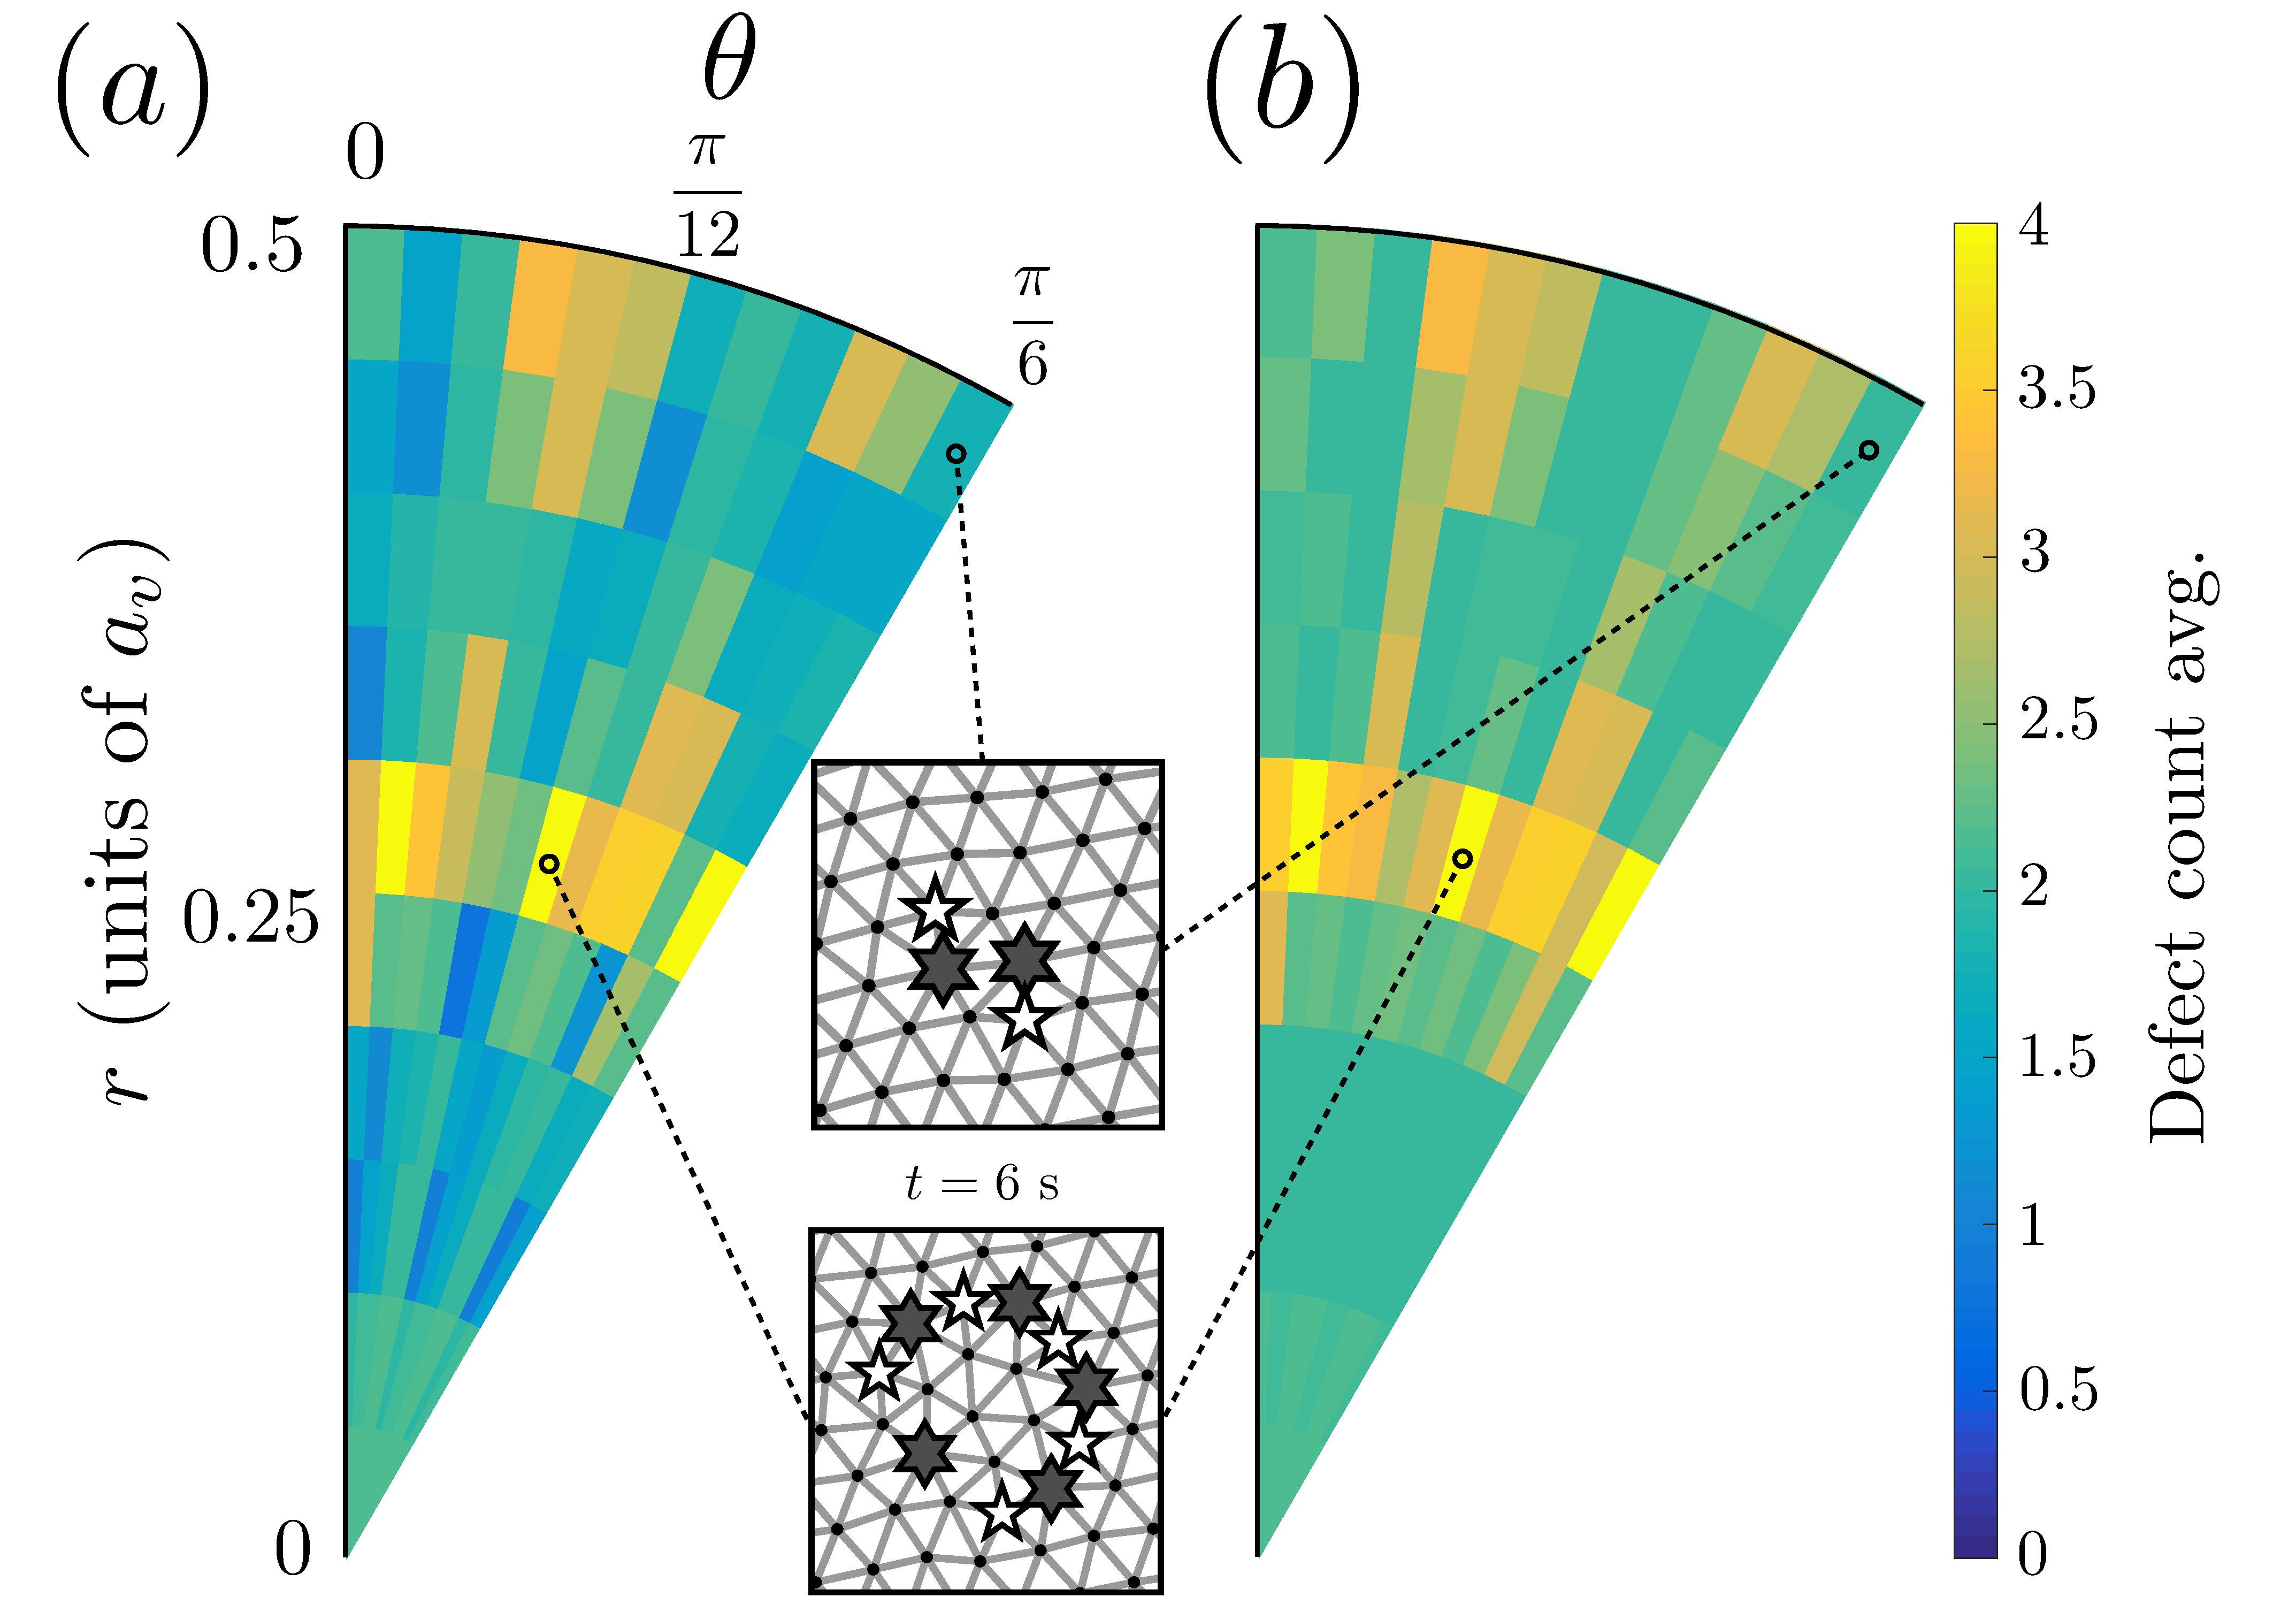
\includegraphics[width=0.7\textwidth]{ch6_phasegineer/arxiv/fig7.pdf}
    \caption{The time-averaged number of defects appearing over a range of imprint positions, relative to a central vortex from $t=1\rightarrow$10 s, and allowing 1 s of settling time. Both 5-fold ($a$) and 7-fold ($b$) defects are shown. The insets show a snapshot of two different parameter regions at $t=6$ s. A high simultaneity is observed between their appearance, where a paired (5,7) defect indicates a lattice dislocation. Not all 5 and 7-fold defects pair, as some can exist individually, or pair with other $n$-fold defects.} \label{fig:lattice_misalign}
\end{figure}

To further demonstrate the localized nature of the defect, let us briefly discuss the situation where two vortices are erased in separate regions away from the lattice centre. The Delaunay triangulation for this case is shown in Fig.~\ref{fig:traj_2vtx_edge}, and the independence of the two localized regions is clearly visible, with each  showing similar behavior to the case discussed above. Since we are limiting ourselves here to perfect imprinting, we also show the number of edges formed between vortices as a function of time for 5, 6 and 7 nearest neighbors respectively ($N_x$) in Fig.~\ref{fig:vtx_rem2_edge}. One can see that the initial perturbation settles quickly to values similar to the ones above.

\begin{figure}[h!]\centering
    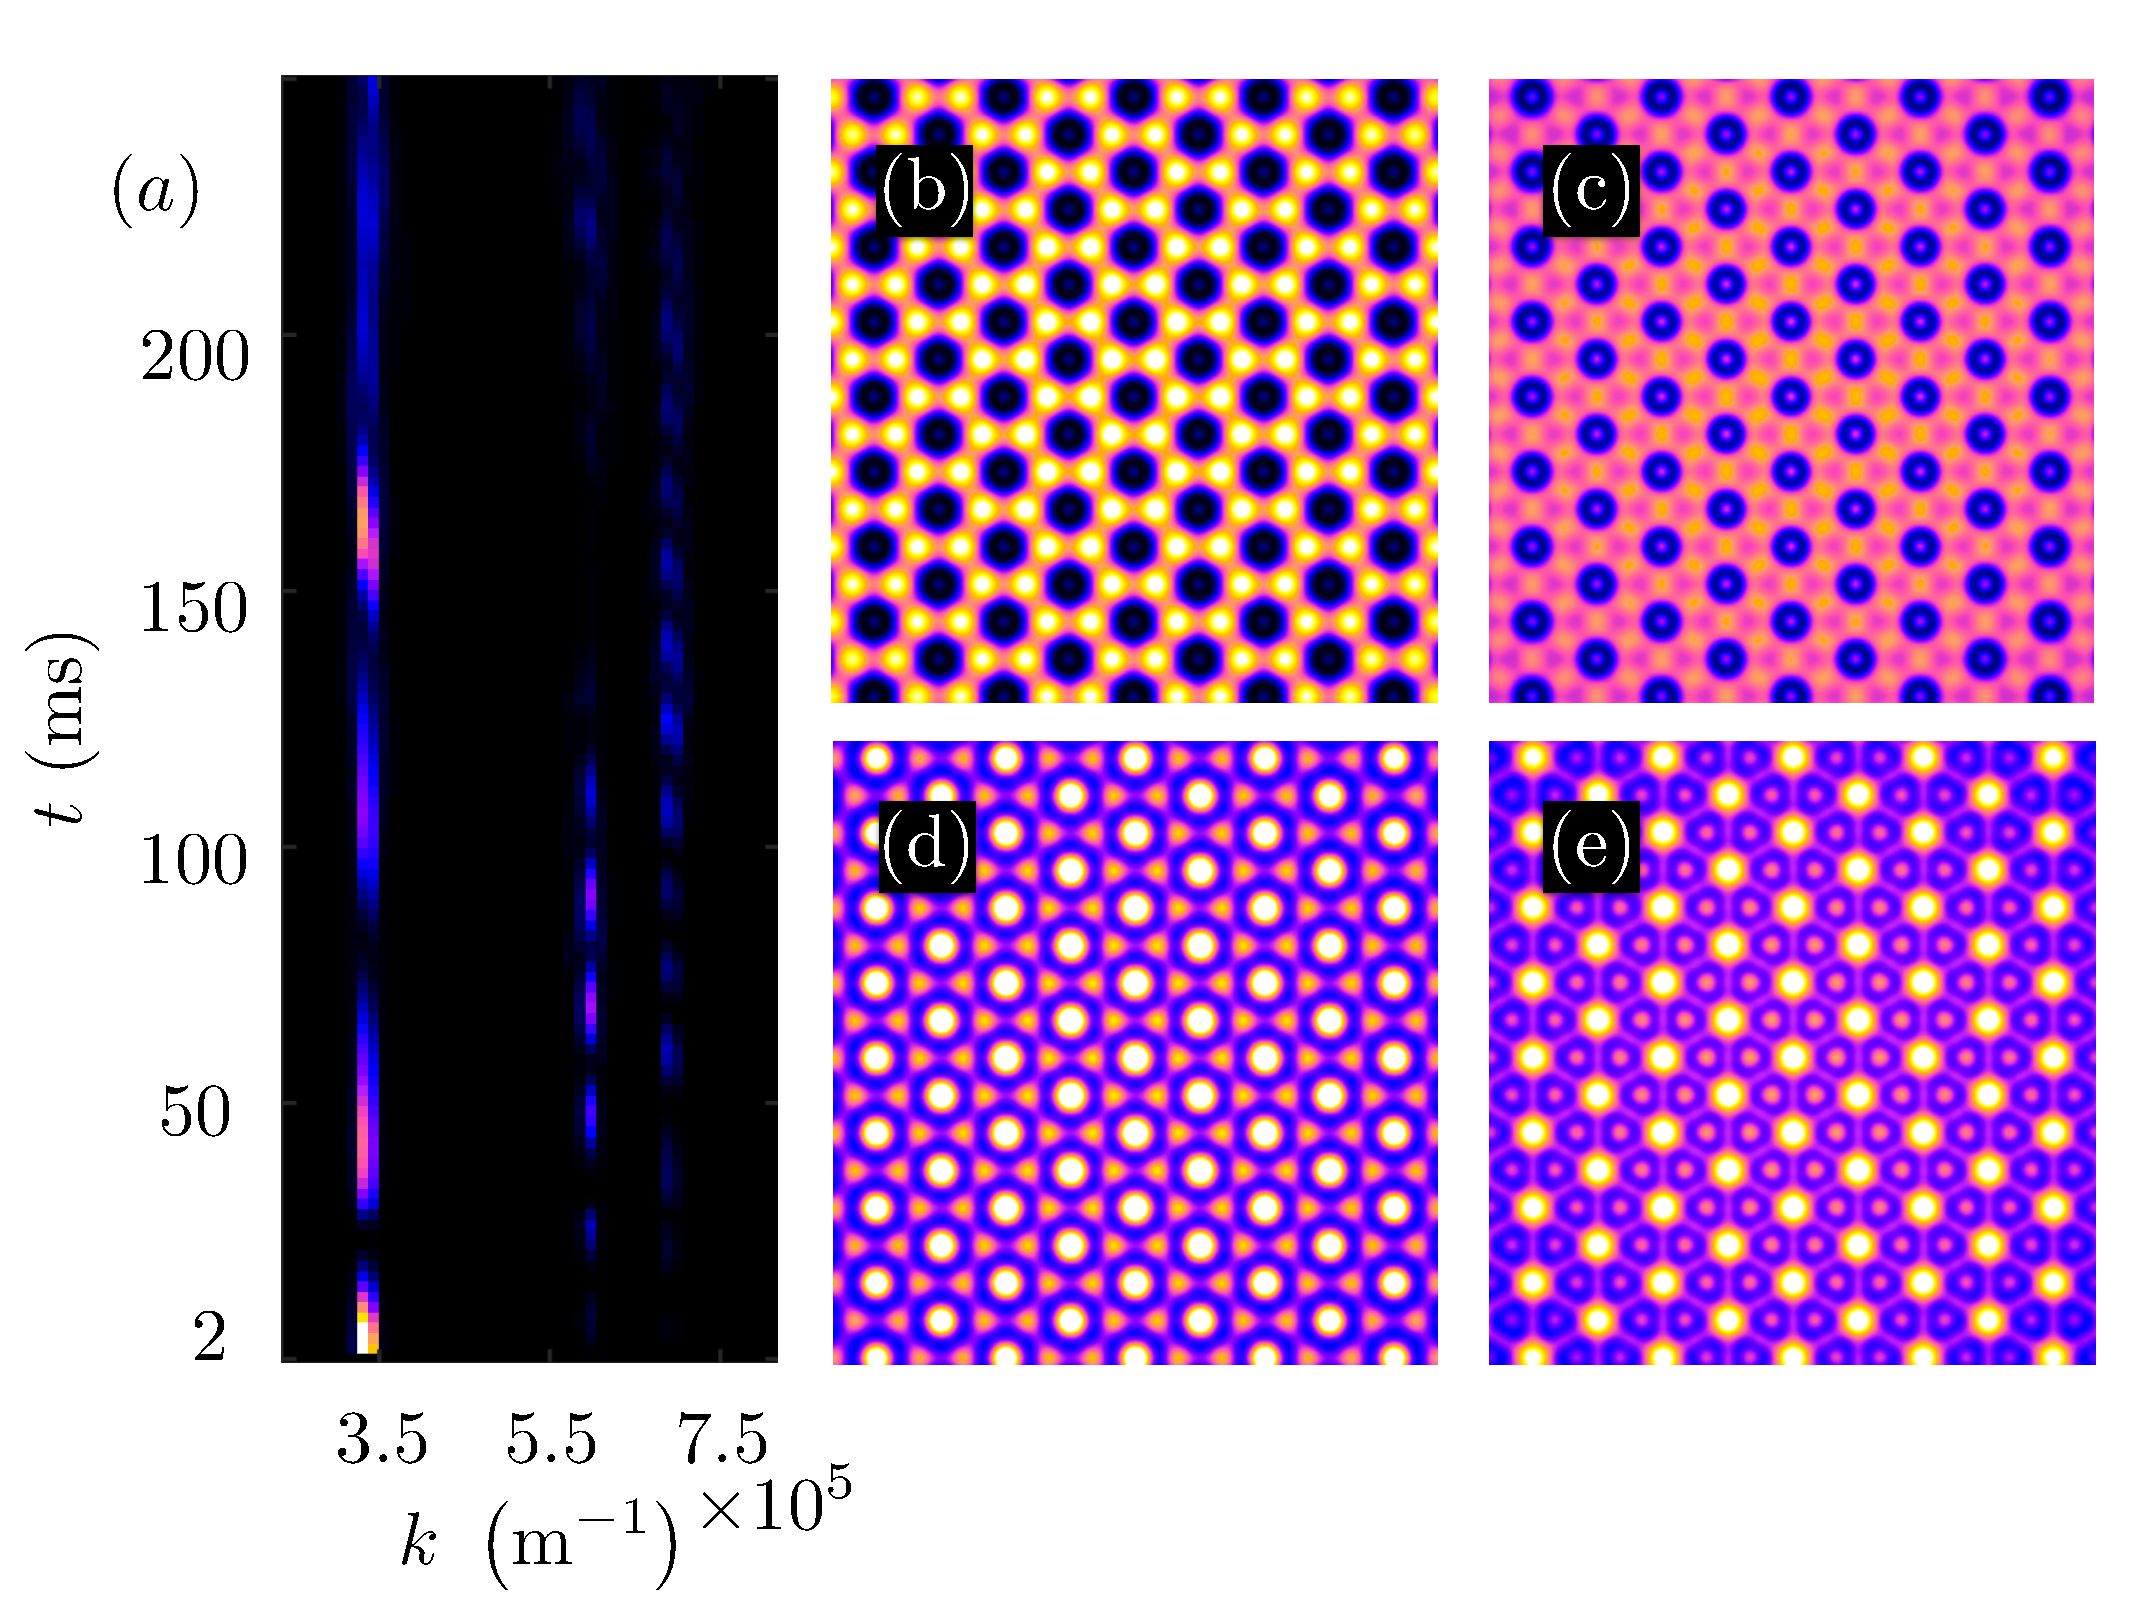
\includegraphics[width=0.7\textwidth]{ch6_phasegineer/arxiv/fig8.pdf}
    \caption{Delaunay triangulation of the vortex lattice upon removal of two vortices at either sides of the lattice for $t=\{0.01,0.8,2,6\}$ s. The resulting defects that form remain localized for long times. The lattice largely remains ordered, as observed with removing the central vortex.}\label{fig:traj_2vtx_edge}
\end{figure}

\begin{figure}[h!]\centering
    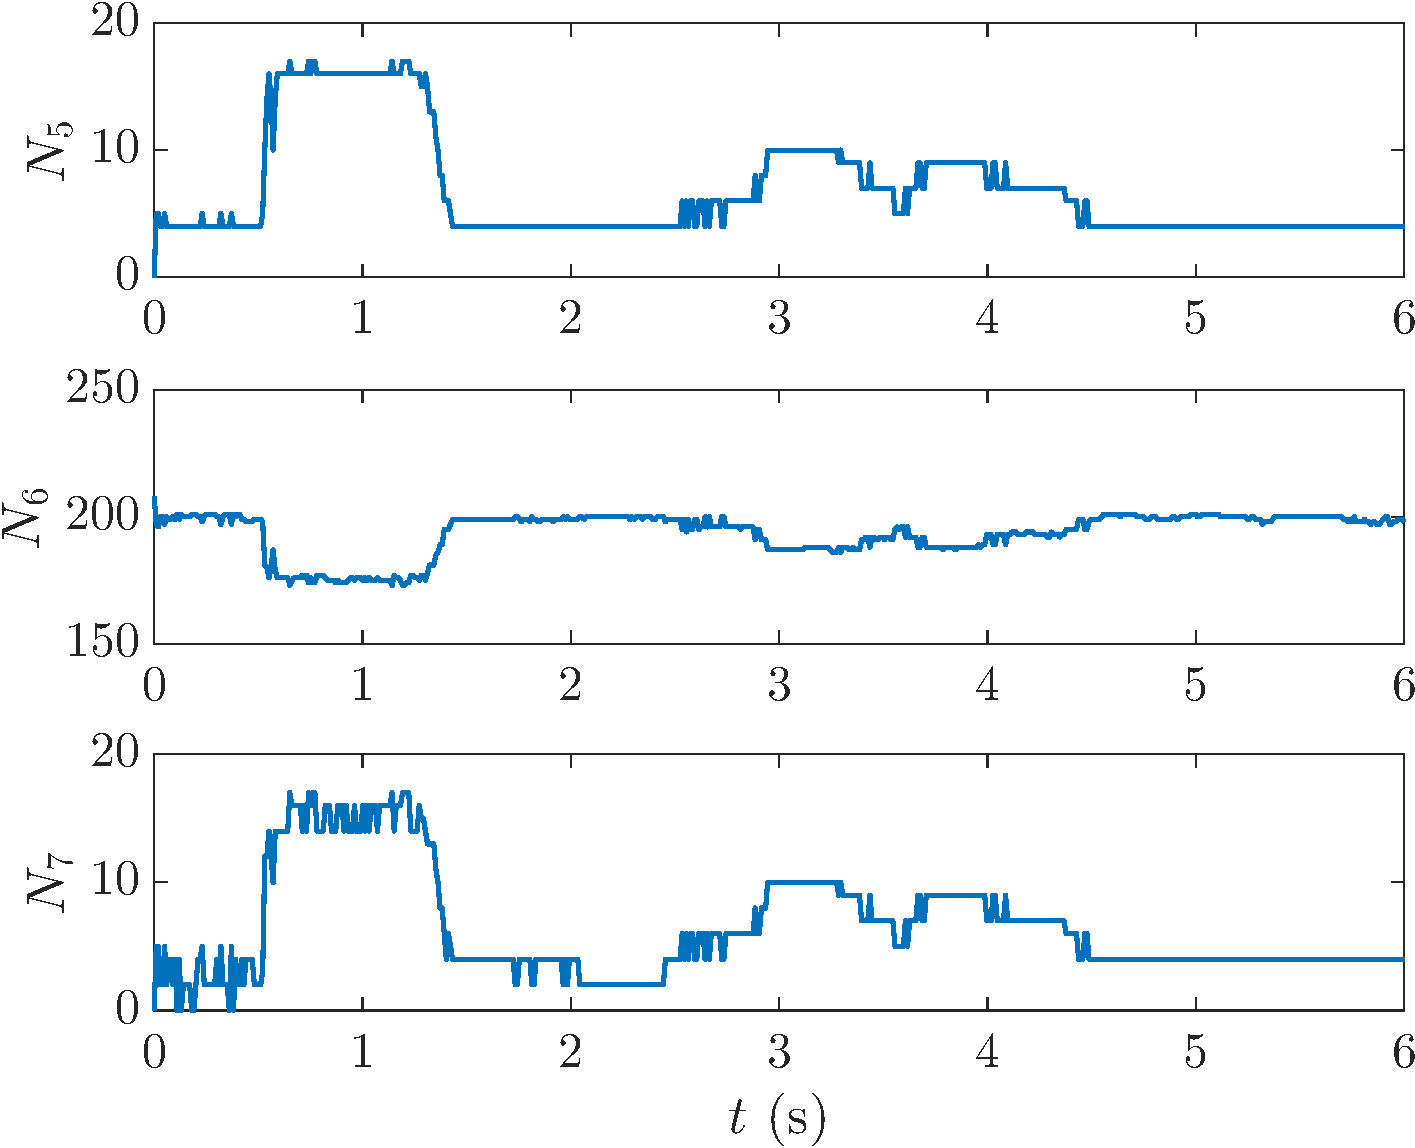
\includegraphics[width=0.7\textwidth]{ch6_phasegineer/arxiv/fig9.pdf}
    \caption{The defect count taken from a Delaunay triangulation of the vortex lattice following the removal of two vortices on opposite sides as a function of time. After a brief settling time, the lattice attains an almost constant defect count.}\label{fig:remove7_defect}
    \label{fig:vtx_rem2_edge}
\end{figure}

%%%%%%%%%%%%%%%%%%%%%%%%%%%%%%%%%%%%%%%%%%%%%%%%%%%%%%%%%%%%%%%%%%%%%%%%%%%%%%%%%%%%%%%%%%%%%%%%%%%%%%%%%%%%%%%%%%%%%%%%%%%%%%%%%%%%%%%%%%%%%
%%%%%%%%%%%%%%%%%%%%%%%%%%%%%%%%%%%%%%%%%%%%%%%%%%%%%%%%%%%%%%%%%%%%%%%%%%%%%%%%%%%%%%%%%%%%%%%%%%%%%%%%%%%%%%%%%%%%%%%%%%%%%%%%%%%%%%%%%%%%%

In addition to simply erasing vorticity, we can also use phase imprinting to create varying degrees of disorder. By, for example, applying an appropriate $4\pi$ magnitude phase imprint we can replace a vortex with an antivortex at a given position. Since this does not require a change in the local density, all resulting perturbations stem from the adjusted velocity field of the vortex that has been flipped \cite{VTX:Madarassy_gfd_2009}. However, it is immediately obvious that such a situation is unstable, which can be confirmed by observing the creation of a large number of defects, as shown in Fig.~\ref{fig:varr161anti_defect}. An increase in the number of defects can be seen up to approximately $t=3$ s, during which the antivortex causes local disordering of the lattice, annihilates with a nearby vortex, and gives rise to the creation of a large number of (5,7) defect pairs. After this the number of defects no longer grows, but instead fluctuates about a stable value which is greater that that of the previously examined cases.

\begin{figure}[h!]\centering
    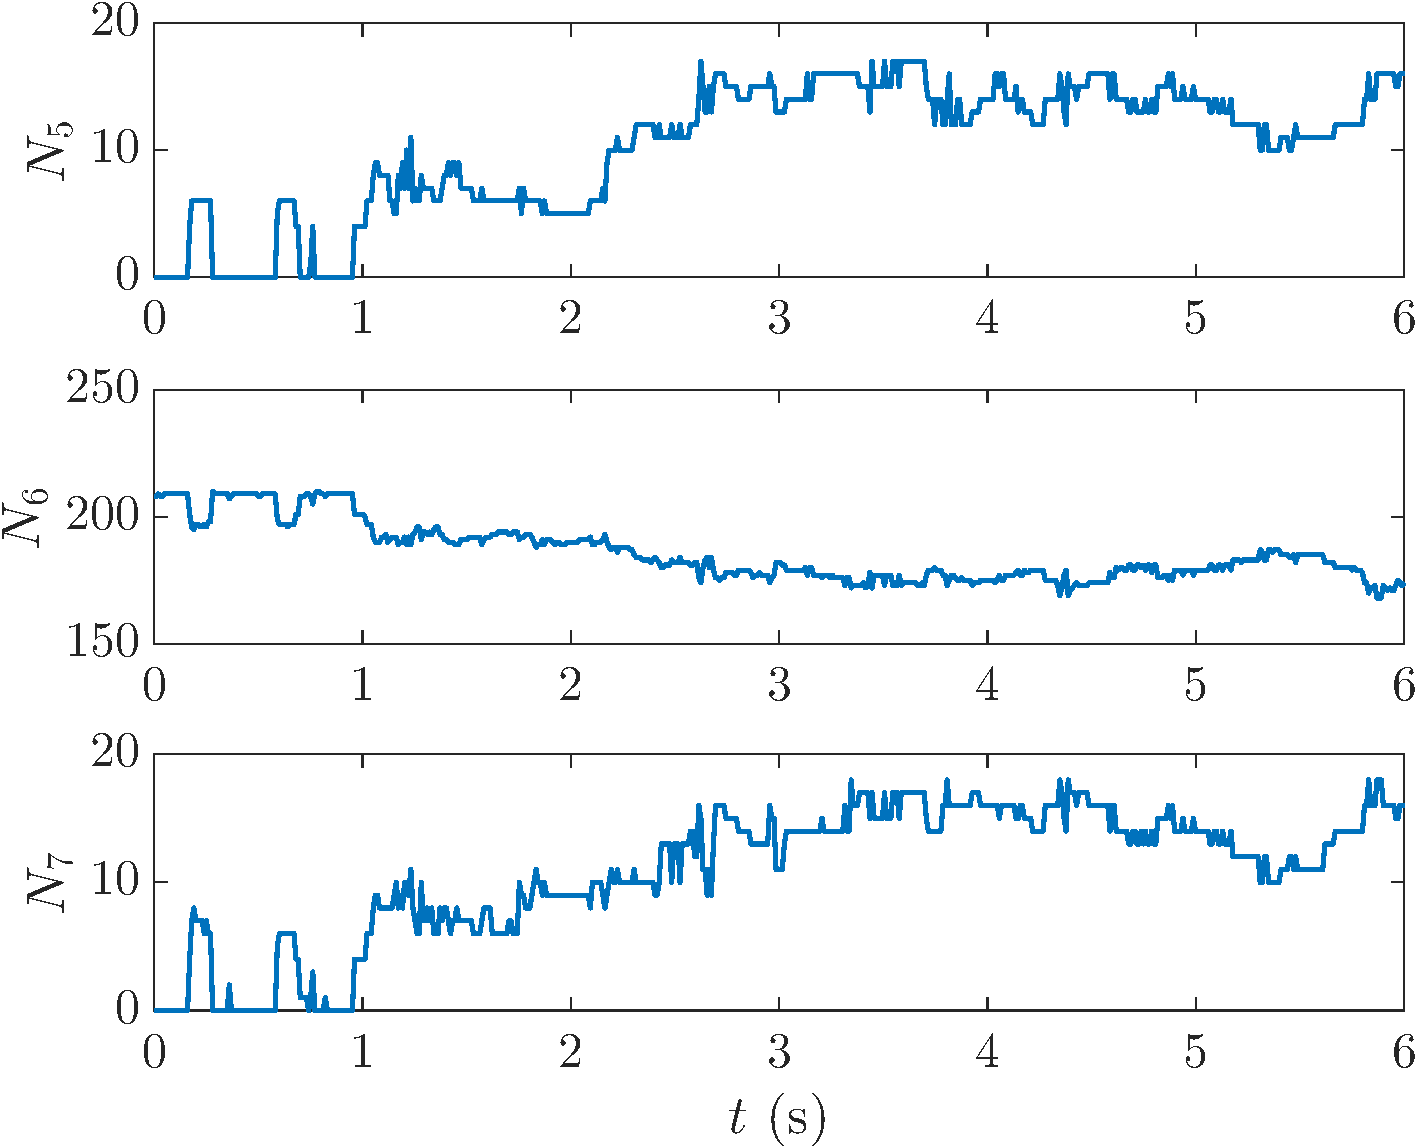
\includegraphics[width=0.7\textwidth]{ch6_phasegineer/arxiv/fig10.pdf}
    \caption{The defect count taken from a Delaunay triangulation of the vortex lattice following an insertion of an antivortex. The number of defects increases as the local structure decays, and eventually gives rise to a quasi-constant state.}\label{fig:varr161anti_defect}
\end{figure}

A final class of possible perturbations is the removal of a cluster of neighboring vortices from the lattice, and in Fig.~\ref{fig:remove7_defect} we show the results from erasing an entire seven vortex unit cell from the condensate. As expected, one can see that the number of lattice defects rises considerably and does not settle during the time over which we can simulate the condensate. In this case, the disordered regions occupy a large area of the lattice and the number of 6-fold connected vortices becomes very low.

\begin{figure}[h!]\centering
    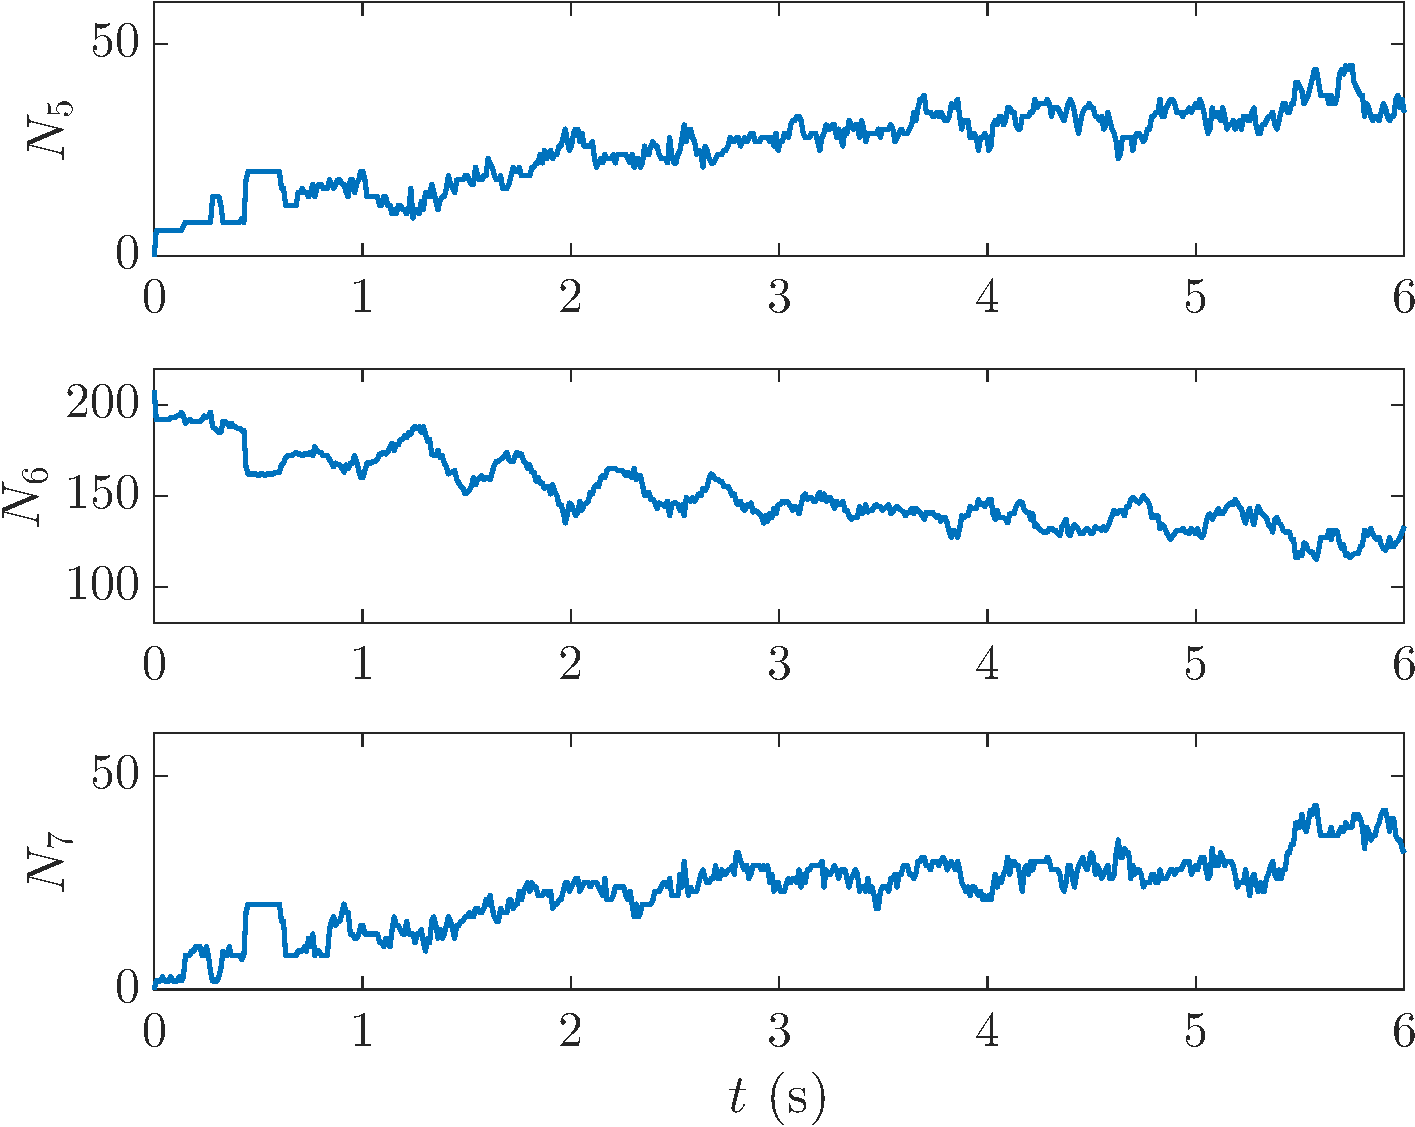
\includegraphics[width=0.7\textwidth]{ch6_phasegineer/arxiv/fig11.pdf}
    \caption{The defect count taken from a Delaunay triangulation of the vortex lattice following the removal of 7 vortices from the centre of the lattice. }\label{fig:remove7_defect}
\end{figure}

Comparing the orientational correlation functions for the three cases discussed in this section (removing two distant vortices, creating an antivortex, and removing 7 vortices) also demonstrates the different degree of disorder they produce (see Fig.~\ref{fig:g6_2edge_anti_nuclear}). The removal of the two vortices at opposite sides of the condensate still yields reasonably high correlations ($\langle g_6(r) \rangle \approx 0.8$) at all times and length scales, indicating a well ordered lattice. Creating an antivortex in the lattice leads to lower correlations across all length scales, especially in the long time limit ($\langle g_6(r) \rangle\approx 0.7$), but still tends to the same long-ranged value as the previous case. This indicates an ordered lattice outside the region of the localized defects. Lastly, the removal of seven vortices shows a significant drop in correlations at all length scales and across both times ($\langle g_6(r) \rangle\approx 0.5$), indicating a global disordering of the vortices, which is consistent with the large number of defects identified earlier.

\begin{figure}[h!]\centering
    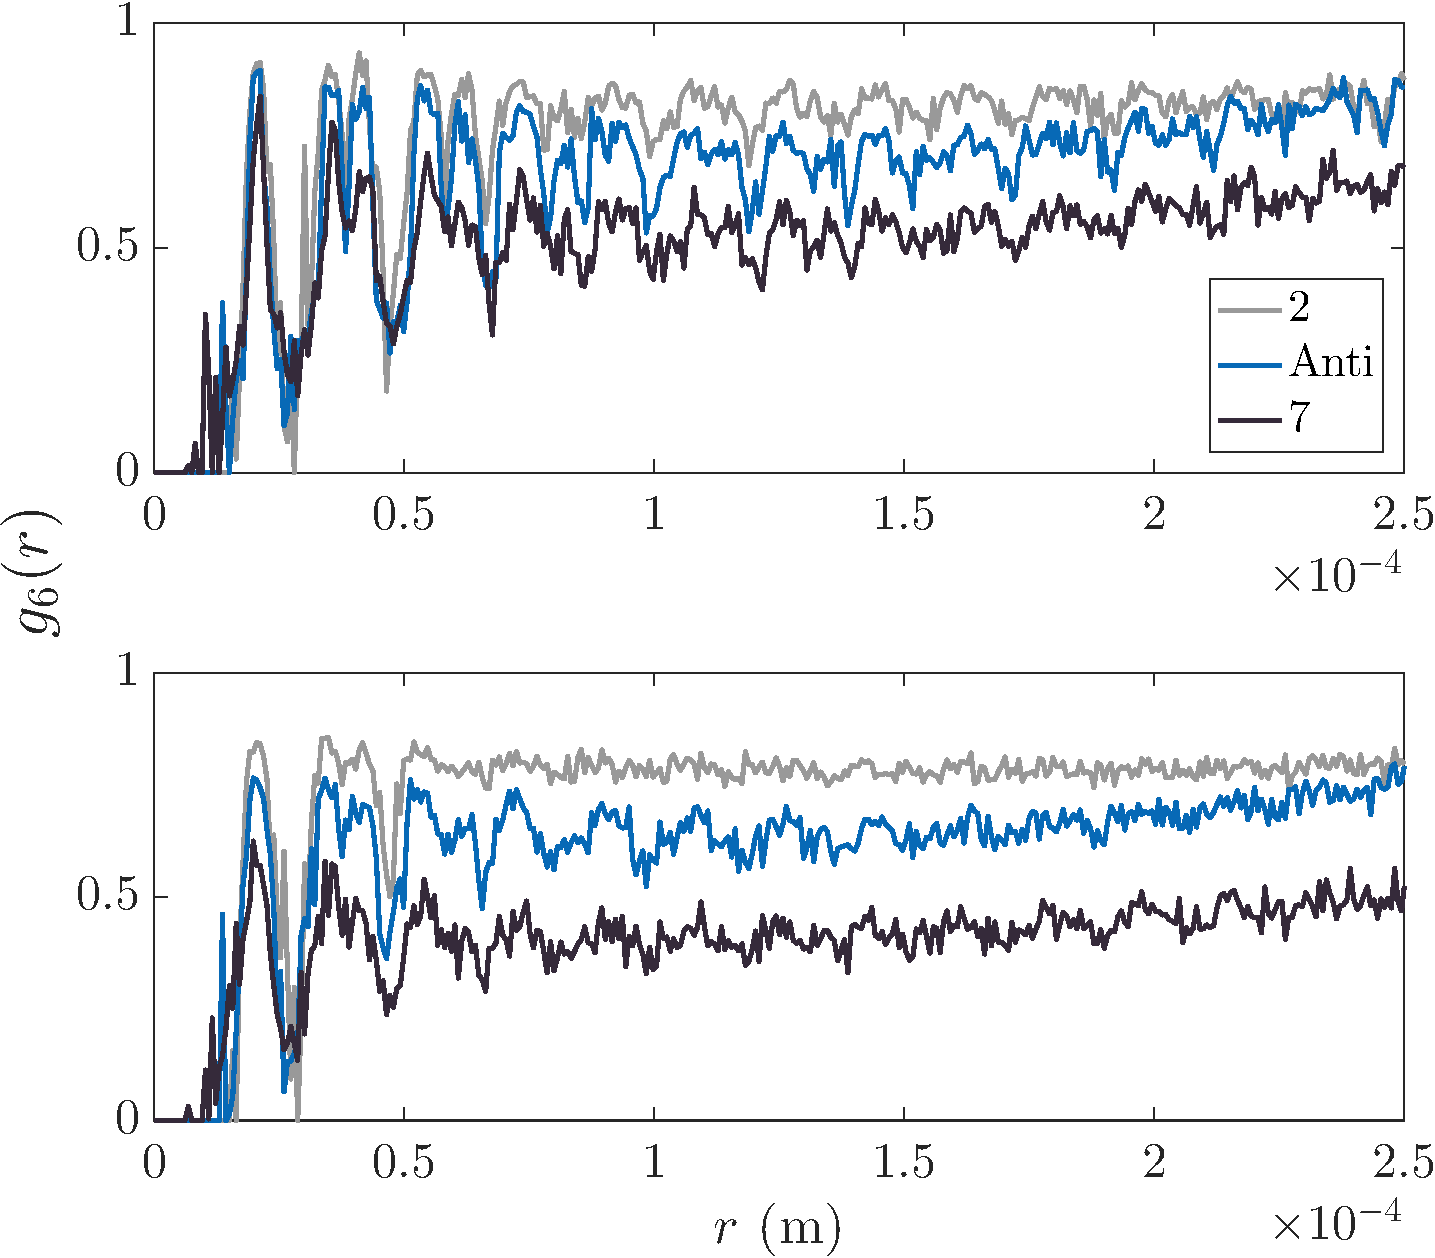
\includegraphics[width=0.7\textwidth]{ch6_phasegineer/arxiv/fig12.pdf}
    \caption{The orientational correlation function is given for moderate ($t=3$ seconds, top) and long ($t=6$ seconds, bottom) times after the phase imprint. The general behaviour at short and long ranges is similar for all three scenarios, but the correlations are significantly reduced, especially for the situation where seven vortices are removed.}\label{fig:g6_2edge_anti_nuclear}
\end{figure}
